
%% bare_conf.tex
%% V1.4b
%% 2015/08/26
%% by Michael Shell
%% See:
%% http://www.michaelshell.org/
%% for current contact information.
%%
%% This is a skeleton file demonstrating the use of IEEEtran.cls
%% (requires IEEEtran.cls version 1.8b or later) with an IEEE
%% conference paper.
%%
%% Support sites:
%% http://www.michaelshell.org/tex/ieeetran/
%% http://www.ctan.org/pkg/ieeetran
%% and
%% http://www.ieee.org/

%%*************************************************************************
%% Legal Notice:
%% This code is offered as-is without any warranty either expressed or
%% implied; without even the implied warranty of MERCHANTABILITY or
%% FITNESS FOR A PARTICULAR PURPOSE! 
%% User assumes all risk.
%% In no event shall the IEEE or any contributor to this code be 
%%liable for
%% any damages or losses, including, but not limited to, incidental,
%% consequential, or any other damages, resulting from the use or misuse
%% of any information contained here.
%%
%% All comments are the opinions of their respective authors and are not
%% necessarily endorsed by the IEEE.
%%
%% This work is distributed under the LaTeX Project Public License (LPPL)
%% ( http://www.latex-project.org/ ) version 1.3, and may be freely used,
%% distributed and modified. A copy of the LPPL, version 1.3, is included
%% in the base LaTeX documentation of all distributions of LaTeX released
%% 2003/12/01 or later.
%% Retain all contribution notices and credits.
%% ** Modified files should be clearly indicated as such, including  **
%% ** renaming them and changing author support contact information. **
%%*************************************************************************


% *** Authors should verify (and, if needed, correct) their LaTeX system  ***
% *** with the testflow diagnostic prior to trusting their LaTeX platform ***
% *** with production work. The IEEE's font choices and paper sizes can   ***
% *** trigger bugs that do not appear when using other class files.       ***                          ***
% The testflow support page is at:
% http://www.michaelshell.org/tex/testflow/



%\documentclass[conference]{IEEEtran}
\documentclass{IEEEtran}
% Some Computer Society conferences also require the compsoc mode option,
% but others use the standard conference format.
%
% If IEEEtran.cls has not been installed into the LaTeX system files,
% manually specify the path to it like:
% \documentclass[conference]{../sty/IEEEtran}





% Some very useful LaTeX packages include:
% (uncomment the ones you want to load)


% *** MISC UTILITY PACKAGES ***
%
%\usepackage{ifpdf}
% Heiko Oberdiek's ifpdf.sty is very useful if you need conditional
% compilation based on whether the output is pdf or dvi.
% usage:
% \ifpdf
%   % pdf code
% \else
%   % dvi code
% \fi
% The latest version of ifpdf.sty can be obtained from:
% http://www.ctan.org/pkg/ifpdf
% Also, note that IEEEtran.cls V1.7 and later provides a builtin
% \ifCLASSINFOpdf conditional that works the same way.
% When switching from latex to pdflatex and vice-versa, the compiler may
% have to be run twice to clear warning/error messages.






% *** CITATION PACKAGES ***
%
%\usepackage{cite}
% cite.sty was written by Donald Arseneau
% V1.6 and later of IEEEtran pre-defines the format of the cite.sty package
% \cite{} output to follow that of the IEEE. Loading the cite package will
% result in citation numbers being automatically sorted and properly
% "compressed/ranged". e.g., [1], [9], [2], [7], [5], [6] without using
% cite.sty will become [1], [2], [5]--[7], [9] using cite.sty. cite.sty's
% \cite will automatically add leading space, if needed. Use cite.sty's
% noadjust option (cite.sty V3.8 and later) if you want to turn this off
% such as if a citation ever needs to be enclosed in parenthesis.
% cite.sty is already installed on most LaTeX systems. Be sure and use
% version 5.0 (2009-03-20) and later if using hyperref.sty.
% The latest version can be obtained at:
% http://www.ctan.org/pkg/cite
% The documentation is contained in the cite.sty file itself.






% *** GRAPHICS RELATED PACKAGES ***
%
\ifCLASSINFOpdf
  % \usepackage[pdftex]{graphicx}
  % declare the path(s) where your graphic files are
  % \graphicspath{{../pdf/}{../jpeg/}}
  % and their extensions so you won't have to specify these with
  % every instance of \includegraphics
  % \DeclareGraphicsExtensions{.pdf,.jpeg,.png}
\else
  % or other class option (dvipsone, dvipdf, if not using dvips). graphicx
  % will default to the driver specified in the system graphics.cfg if no
  % driver is specified.
  % \usepackage[dvips]{graphicx}
  % declare the path(s) where your graphic files are
  % \graphicspath{{../eps/}}
  % and their extensions so you won't have to specify these with
  % every instance of \includegraphics
  % \DeclareGraphicsExtensions{.eps}
\fi
% graphicx was written by David Carlisle and Sebastian Rahtz. It is
% required if you want graphics, photos, etc. graphicx.sty is already
% installed on most LaTeX systems. The latest version and documentation
% can be obtained at: 
% http://www.ctan.org/pkg/graphicx
% Another good source of documentation is "Using Imported Graphics in
% LaTeX2e" by Keith Reckdahl which can be found at:
% http://www.ctan.org/pkg/epslatex
%
% latex, and pdflatex in dvi mode, support graphics in encapsulated
% postscript (.eps) format. pdflatex in pdf mode supports graphics
% in .pdf, .jpeg, .png and .mps (metapost) formats. Users should ensure
% that all non-photo figures use a vector format (.eps, .pdf, .mps) and
% not a bitmapped formats (.jpeg, .png). The IEEE frowns on bitmapped formats
% which can result in "jaggedy"/blurry rendering of lines and letters as
% well as large increases in file sizes.
%
% You can find documentation about the pdfTeX application at:
% http://www.tug.org/applications/pdftex





% *** MATH PACKAGES ***
%
\usepackage{amssymb} %new add for \triangleq

\usepackage[cmex10]{amsmath}
%\usepackage{amsmath}
% A popular package from the American Mathematical Society that provides
% many useful and powerful commands for dealing with mathematics.
%
% Note that the amsmath package sets \interdisplaylinepenalty to 10000
% thus preventing page breaks from occurring within multiline equations. Use:
%\interdisplaylinepenalty=2500
% after loading amsmath to restore such page breaks as IEEEtran.cls normally
% does. amsmath.sty is already installed on most LaTeX systems. The latest
% version and documentation can be obtained at:
% http://www.ctan.org/pkg/amsmath



\usepackage{listings}

% *** SPECIALIZED LIST PACKAGES ***
%
\usepackage{algorithmic}
% algorithmic.sty was written by Peter Williams and Rogerio Brito.
% This package provides an algorithmic environment fo describing algorithms.
% You can use the algorithmic environment in-text or within a figure
% environment to provide for a floating algorithm. Do NOT use the algorithm
% floating environment provided by algorithm.sty (by the same authors) or
% algorithm2e.sty (by Christophe Fiorio) as the IEEE does not use dedicated
% algorithm float types and packages that provide these will not provide
% correct IEEE style captions. The latest version and documentation of
% algorithmic.sty can be obtained at:
% http://www.ctan.org/pkg/algorithms
% Also of interest may be the (relatively newer and more customizable)
% algorithmicx.sty package by Szasz Janos:
% http://www.ctan.org/pkg/algorithmicx




% *** ALIGNMENT PACKAGES ***
%
\usepackage{array}
% Frank Mittelbach's and David Carlisle's array.sty patches and improves
% the standard LaTeX2e array and tabular environments to provide better
% appearance and additional user controls. As the default LaTeX2e table
% generation code is lacking to the point of almost being broken with
% respect to the quality of the end results, all users are strongly
% advised to use an enhanced (at the very least that provided by array.sty)
% set of table tools. array.sty is already installed on most systems. The
% latest version and documentation can be obtained at:
% http://www.ctan.org/pkg/array


% IEEEtran contains the IEEEeqnarray family of commands that can be used to
% generate multiline equations as well as matrices, tables, etc., of high
% quality.




% *** SUBFIGURE PACKAGES ***
%\ifCLASSOPTIONcompsoc
%  \usepackage[caption=false,font=normalsize,labelfont=sf,textfont=sf]{subfig}
%\else
%  \usepackage[caption=false,font=footnotesize]{subfig}
%\fi
% subfig.sty, written by Steven Douglas Cochran, is the modern replacement
% for subfigure.sty, the latter of which is no longer maintained and is
% incompatible with some LaTeX packages including fixltx2e. However,
% subfig.sty requires and automatically loads Axel Sommerfeldt's caption.sty
% which will override IEEEtran.cls' handling of captions and this will result
% in non-IEEE style figure/table captions. To prevent this problem, be sure
% and invoke subfig.sty's "caption=false" package option (available since
% subfig.sty version 1.3, 2005/06/28) as this is will preserve IEEEtran.cls
% handling of captions.
% Note that the Computer Society format requires a larger sans serif font
% than the serif footnote size font used in traditional IEEE formatting
% and thus the need to invoke different subfig.sty package options depending
% on whether compsoc mode has been enabled.
%
% The latest version and documentation of subfig.sty can be obtained at:
% http://www.ctan.org/pkg/subfig




% *** FLOAT PACKAGES ***
%
%\usepackage{fixltx2e}
% fixltx2e, the successor to the earlier fix2col.sty, was written by
% Frank Mittelbach and David Carlisle. This package corrects a few problems
% in the LaTeX2e kernel, the most notable of which is that in current
% LaTeX2e releases, the ordering of single and double column floats is not
% guaranteed to be preserved. Thus, an unpatched LaTeX2e can allow a
% single column figure to be placed prior to an earlier double column
% figure.
% Be aware that LaTeX2e kernels dated 2015 and later have fixltx2e.sty's
% corrections already built into the system in which case a warning will
% be issued if an attempt is made to load fixltx2e.sty as it is no longer
% needed.
% The latest version and documentation can be found at:
% http://www.ctan.org/pkg/fixltx2e


%\usepackage{stfloats}
% stfloats.sty was written by Sigitas Tolusis. This package gives LaTeX2e
% the ability to do double column floats at the bottom of the page as well
% as the top. (e.g., "\begin{figure*}[!b]" is not normally possible in
% LaTeX2e). It also provides a command:
%\fnbelowfloat
% to enable the placement of footnotes below bottom floats (the standard
% LaTeX2e kernel puts them above bottom floats). This is an invasive package
% which rewrites many portions of the LaTeX2e float routines. It may not work
% with other packages that modify the LaTeX2e float routines. The latest
% version and documentation can be obtained at:
% http://www.ctan.org/pkg/stfloats
% Do not use the stfloats baselinefloat ability as the IEEE does not allow
% \baselineskip to stretch. Authors submitting work to the IEEE should note
% that the IEEE rarely uses double column equations and that authors should try
% to avoid such use. Do not be tempted to use the cuted.sty or midfloat.sty
% packages (also by Sigitas Tolusis) as the IEEE does not format its papers in
% such ways.
% Do not attempt to use stfloats with fixltx2e as they are incompatible.
% Instead, use Morten Hogholm'a dblfloatfix which combines the features
% of both fixltx2e and stfloats:
%
% \usepackage{dblfloatfix}
% The latest version can be found at:
% http://www.ctan.org/pkg/dblfloatfix




% *** PDF, URL AND HYPERLINK PACKAGES ***
%
\usepackage{url}
\usepackage{float}
% url.sty was written by Donald Arseneau. It provides better support for
% handling and breaking URLs. url.sty is already installed on most LaTeX
% systems. The latest version and documentation can be obtained at:
% http://www.ctan.org/pkg/url
% Basically, \url{my_url_here}.




% *** Do not adjust lengths that control margins, column widths, etc. ***
% *** Do not use packages that alter fonts (such as pslatex).         ***
% There should be no need to do such things with IEEEtran.cls V1.6 and later.
% (Unless specifically asked to do so by the journal or conference you plan
% to submit to, of course. )

\ifCLASSOPTIONcompsoc
\usepackage[caption=false,font=normalsize,labelfon
t=sf,textfont=sf]{subfig} \else
\usepackage[caption=false,font=footnotesize]{subfi
g} \fi
\usepackage{mdwmath}
\usepackage{mdwtab}
\usepackage{multirow}
\usepackage[ruled,vlined]{algorithm2e}
\usepackage{graphicx}
\usepackage{epstopdf}

\newcommand{\figwidth}{0.75\linewidth}
\newcommand{\figwidthsmall}{0.5\linewidth}
\newcommand{\figwidtha}{0.7\linewidth}
\newcommand{\figwidthb}{0.80\linewidth}
\newcommand{\figwidthdouble}{0.5\linewidth}
\newcommand{\figwidthtriple}{0.32\linewidth}
\def\figref#1{Fig.~\ref{#1}}
\def\secref#1{Section~\ref{#1}}
\def\tabref#1{Table~\ref{#1}}
%\DeclareMathOperator{\sgn}{sgn}
%\DeclareMathOperator{\num}{num}
%\DeclareMathOperator{\erf}{erf}
%\DeclareMathOperator{\mean}{mean}
%\DeclareMathOperator{\Cov}{Cov}
%\DeclareMathOperator{\E}{E}
%\DeclareMathOperator{\Var}{Var}
\DeclareMathOperator{\trace}{trace}
%\DeclareMathOperator{\tr}{tr}

% correct bad hyphenation here
\hyphenation{op-tical net-works semi-conduc-tor}


\begin{document}

%
% paper title
% Titles are generally capitalized except for words such as a, an, and, as,
% at, but, by, for, in, nor, of, on, or, the, to and up, which are usually
% not capitalized unless they are the first or last word of the title.
% Linebreaks \\ can be used within to get better formatting as desired.
% Do not put math or special symbols in the title.
\title{Connected and Robotic Autonomous System}


% author names and affiliations
\author{\IEEEauthorblockN{Jay Sureshbhai Parsana, Prashant Shushilbhai Gandhi, Saumil Parag Shah, Vatsal Kirit Makani} \\
 \IEEEauthorblockA{Computer Engineering Department\\
 San Jos\'{e} State University (SJSU)\\
 San Jos\'{e}, CA, USA \\
 Email: \{jay.parsana, prashantshushilbhai.gandhi, saumil.shah, vatsalkirit.makani\}@sjsu.edu}
 }
 
% make the title area
\maketitle

% As a general rule, do not put math, special symbols or citations
% in the abstract
\begin{abstract}
Nowadays autonomous robotic systems are the main focus of research in the tech industry. The project, connected and autonomous system, is an amalgam of embedded systems, IoT, distributed sensor networks, and deep learning applications. In this project, we aim to develop a drone that has autonomous capabilities and can track moving objects such as vehicles and people. Its application will be to capture videos or images of these moving objects autonomously. The ultrawide beacon, RTK GPS, and a stereoscopic camera will be attached to the drone for tracking the object. The object is embedded with a beacon and an RTK GPS so that the drone can keep track of that object. 
\newline The low-level architecture is based on NuttX OS, with ArduPilot firmware, and Pixhawk 4 flight controller. The higher-level architecture uses Linux based systems that can support complex frameworks and computing-intensive applications such as object detection, classification, and system localization. The system makes use of a ZED stereo camera to get the depth information from the disparity map for autonomous landing and obstacle avoidance. We are making use of datasets that are relevant to train our deep learning models and avoid obstacles while in mid-air.

\end{abstract}

% no keywords
\begin{IEEEkeywords}
Ardupilot, autonomous, deep learning, localization, object detection, obstacle avoidance, Pixhawk 4, RTK GPS, stereo camera, tracking, ultrawide-band beacon
\end{IEEEkeywords}



\IEEEpeerreviewmaketitle



\section{Introduction}\label{sec:introduction}
In the past few decades, autonomous robotics has made a fine share of advancements in the tech industry and continues to improve every day with the applications, not only restricted for industrial purposes but also making the step forward towards other applications where it is inefficient, impossible and dangerous for human intervention. This has been possible because of drastic improvements and support for the machine learning algorithms. Robotic systems are the amalgam of mechanical engineering, electronics engineering, and computer science. “Research by the Japan Robotics Association (JPA), the United Nations Economic Commission (UNEC), and the International Federation of Robotics (IFR), indicates that the market growth for personal robots, including those used for entertainment and educational purposes, has been tremendous and this trend may continue over the coming decades” [1]. With the advancement of AI and Machine learning, robotic systems have become autonomous. The word “connected” comes from the fact that these systems can have IoT capabilities that can send data for monitoring and storage over to the cloud. Our paper is focused more on drones and we thus restrict the discussion of the generic robotic system towards that area.
\newline Drones are the nickname for unmanned aerial vehicles (UAV) which can be used for various domestic to critical applications. Lian Pin Koh and Serge A. Wich (2012) explains the use of “unmanned aerial vehicles for surveying and mapping forests and biodiversity for environmental and conservation applications, which include near-real-time mapping of local land cover, monitoring of illegal forest activities (e.g., logging, fires), and surveying of large animal species” [2]. The authors' Author Milan Erdelj, Michał Król, EnricoNatalizio (2017) explain the importance of drones to help the rescue services to operate efficiently at an event of natural disaster [3]. Such applications make drones, one of the useful and popular robotic systems. The drones can come in various shapes and sizes and can be used for recreational applications such as “hobby purposes while being flown in a park to take photographs from unusual perspectives and angles. It can also be used for a commercial application such as business for surveillance, domestic policing, the delivery of goods and for oil, gas, and mineral exploration. Military applications would be drones that are used for a variety of purposes such as reconnaissance, surveillance, remote sensing, armed attacks and warfare” [4]. The drones can be either remote-controlled from the ground station or made autonomous with the help of programming.
\newline For unsupervised navigation, autonomous drones require several sensors that work together to navigate and detect obstacles. In surveillance applications, autonomous drones make use of deep learning models that are useful for detecting the objects and tracking their movements. The authors Ludovic Apvrille, Tullio Tanzi, and Jean-Luc Dugelay (2014) explain the use of Sparse3D and HOG Algorithm to detect objects and avoid obstacles providing a faster response [5]. However, their system requires an efficient autonomy to manage energy, fix the hardware-software configurations, and use the system in critical situations [5]. This paper explains our project implementation of a “connected and autonomous drone system” to counter these problems.
\newline To fix the hardware-software configuration issues, we propose a two-level architecture, where low-level architecture takes care of the sensing units to detect and avoid obstacles using proximity sensors such as ultrasonic sensors. The stereo camera setup is used to measure the distance to the objects. This is done by generating disparity between the left and right images and extracting a depth map from it. The high-level architecture is trained by complex deep learning models to track the objects to be monitored and collect the data to be sent to the cloud. To monitor the drone navigation at outdoor conditions, GPS modules can be used to pinpoint the exact coordinates of the drone. There is a possibility that drone needs to perform indoor navigation and GPS module would not work. To overcome such a scenario, we are using an ultrawide-band beacon (UWB) to get the exact drone location indoors. We aim to achieve autonomous capability by incorporating the Ardupilot on the PixHawk4 platform. The Ardupilot platform has really good support for drone applications with features such as data-logging, analysis, simulation tools, etc. [6]. Since it is an open-source platform, it has a huge ecosystem of sensors, communication protocols, and compatible hardware/computers [6].

\section{Related Works}\label{sec:related}
There are many autonomous systems research going on that can be used as a reference to develop our project. For an indoor autonomous system, Zhengang Li, Yong Xiong, Lei Zhou (2017) explains the working of the indoor wheelchair performing the autonomous exploration based on inexpensive RGB camera and ROS. The authors explain that the wheelchair rotary systems are controlled by the robot operating system in the host computer and RGB camera is used for depth perception, indoor path planning, and obstacle avoidance [7]. The Arduino microcontroller is then used to receive the data from the camera and ROS and accordingly sets the PWM signals for the motors controlling the navigation of the wheelchair.
\newline Some of the airborne automated systems require navigation control based on IMU sensor units like accelerometers, magnetometer, gyroscope, etc. integrated along with location data. Jan Wendel, Oliver Meister, Christian Schlaile, Gert F. Trommer (2006) explain an integrated navigation system for an airborne robotic system that uses GPS and MEMS IMU sensors [8]. The authors propose the solutions for two scenarios: first when GPS data is available and second when GPS is lost [8]. Another replacement for GPS can be an ultrasonic beacon which can be used for indoor positioning. Dongho Kang and Young-Jin Cha (2018) explains the use of ultrasonic beacon in the scenarios where GPS fails to work for a UAVs. The authors explain the application of a “deep convolutional neural network (CNN) for damage detection and a geotagging method for the localization of damage” [9]. “Localization, mapping, and path planning” are the most important algorithms used for any system to be autonomous. Localization, motion planning, and path planning play an important role in deciding the shortest path that any autonomous system can travel in minimum time [10].
\newline The paper [14] describes object detection and tracking for Drones such as Parrot AR drone. It uses an SSD CNN model for object detection. SSD model provides the performance of the Yolo model and accuracy of Region-based object detection models such as Fast-RCNN. A front camera takes a Real-Time image of an object and passes the image to a computer through a Wi-Fi interface. The computer computers the distance and position of the object in real-time and sends the roll, pitch, yaw, and altitude values as parameters to the drone. The drone on receiving these values updates its flight information.
\newline Another paper [15] describes object detection using Qualcomm Snapdragon processor 801.  This development used PX4 Autopilot open-source software to manage the overall operation of the drone. Robot Operating System (ROS) is deployed on ARM core to provide Linux OS support of real-time object detection. The object tracking method uses a lightweight machine learning model and inertial measurement unit data, global positioning system data to calculate the relative distance between the drone the object in a Coordinate based system.
The ultrawideband beacon used in our project is to monitor the tracking of the autonomous drone that shall be used for the remote locations where GPS coordinates cannot be read from the GPS sensor. There are previous implementations of UWB beacon that was used for various applications. The authors' Vincent Mai, Mina Kamel, Matthias Krebs, Andreas Schaffner, Daniel Meier, Liam Paull, and Roland Siegwart(2018) explained the use of UWB sensors integrated with the gyroscope which was used to create an estimator that accurately tracked the position, altitude, linear and angular velocities. “This estimator uses a complete dynamics model, which allows external disturbance estimation. However, it cannot track external forces” and need more strong assumptions for developing hardware and software platforms [12].
Another case study of using UWB technology was the development of a flight system based on the indoor positioning feature. The authors Zhiyuan Shi, Hanbo Li, Hezhi Lin, Lianfen Huang (2018) explains this application. The system was deployed on a Nano quadcopter and indoor navigation was achieved with the help of a UWB indoor positioning system and a flight control scripts. As the author explains, “The accuracy of the UWB indoor positioning system is 10cm which can meet the demands for the nano-quadcopters to perform a formation flight.”[13].The limitation of this system is that it is applicable only for domestic purposes and hobbyists' implementation. To develop a system for industrial or any military applications, we need to deploy strong embedded hardware to achieve the goals.
\newline For this project, we are making use of a stereo camera which will provide us with the depth estimation of an object that is in front of the camera. A disparity map is nothing but the difference in the pixels between the left and the right images. The higher the pixel difference, the greater is the distance from the camera. This is because the stereo camera has two cameras separated by a distance called baseline just like the humans can percept depth because of 2 eyes that create a disparity. The paper [11], formulates a CNN network called Pyramid Stereo Matching Network for generating a disparity map which is quite accurate. It takes into account many different datasets such as KITTI and Scene Flow to evaluate the performance of their network.

\section{Project Architecture}\label{sec:problem}
The project architectre is divided into two parts, Hardware Aspects and Software Aspects. The software aspects furthermore consists of low-level architecture and high-level architecture. The high-level architecture consists of object detection, depth sensing and ultrawideband beacon localization.

\subsection{Hardware Aspects}
We have used the DJI F450 Quadcopter X frame for this project. We are using Emax MT2213-935KV brushless motor which supports 20A to 30A ESCs, LittleBee BLHeils 30A ESC which supports 2-6s batteries. For the autopilot system, we are using Pixhawk 4 mini open source autopilot hardware which uses NuttX OS and PX4 or Ardupilot autopilot firmware. For the live location of drone, we are using ublox GPS which comes with Pixhawk 4 mini. To control the drone remotely, we are using the FrSky Taranis Q X7 radio transmitter and x8r receiver at the drone side. For high-level architecture, we are using NVIDIA Jetson nano and Zed camera for object avoidance. We have 3D printed support for jetson nano. Two different batteries are required to power Pixhawk 4 min and jetson nano. One battery is powering all ESCs, GPS, and Pixhawk 4 mini through the PM06 V2 power management module.

\begin{figure}[htb]
\centering
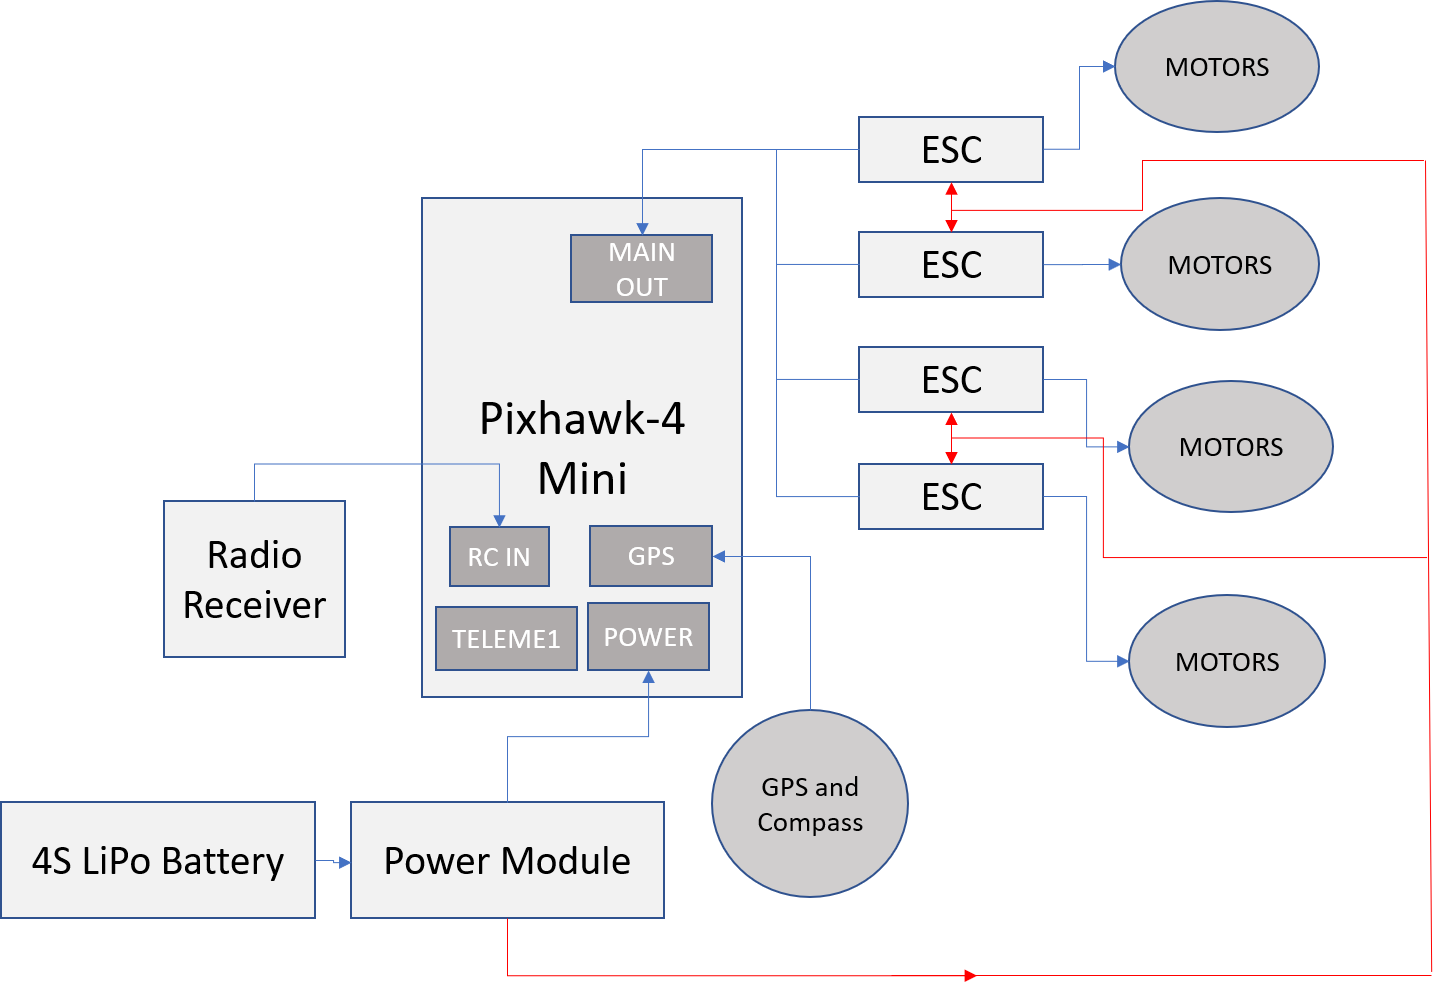
\includegraphics[width=1\linewidth]{fig/hardware_connection.png}
\caption{Hardware connection fliow diagram.} \label{fig.structure}
\end{figure}

\subsection{Software Aspects}
The software aspect of our project is divided into the higher level and lower level architecture as follows:

\begin{figure}[htb]
\centering
\includegraphics[width=1\linewidth]{fig/block_diagram.png}
\caption{System Architecture.} \label{fig.structure}
\end{figure}

\subsubsection{Low-Level Architecture}
The low-level architecture is illustrated as the right block of the system architecture in the Fig. 2. This architecture is composed of Piwhawk Microcontroller which is the main controller to manage the flight of the drone. It connected to different sensors through the CAN bus. The compass is used to provide the heading angle and direction for the flight of the drone. The IMU (Intertial measurement unit) sensors consist of accelerometer and gyroscope providing the tilt and rotational information data for managing the yaw, pitch, and roll. The GPS provides the positional information of the drone in terms of the earth’s latitude and longitude to track its real-time location. The motors drive the propellers of the drone allowing the drone to fly. The flight controller i.e. Piwhawk receives these sensors values and takes appropriate action the control the flight of the drone. The Piwhawk 4 mini runs the Ardupilot firmware, which is open-sourced and modified according to the requirement of the drone. The Piwhawk receives flight commands from the flight controller such as QGC station through a wireless communication channel such as MAVLINK at a certain radiofrequency.

\subsubsection{High-Level Architecture}
The high-level architecture has three main components: Jetson Nano controller, UWB (Ultra-wideband) module for indoor localization and ZED capture to capture images from a live video stream. The Jetson Nano is Linux based high computing embedded controller. It has a powerful CPU, GPU cores, much different communication peripheral, and camera support. The UWB sensor computes the location information of the drone wrt to the anchor tags as a reference in terms of X, Y, Z coordinates. The ZED camera on capturing images in front of the drones provides it to a machine learning model in the Jetson Nano, which detects and finds the objects in front of the drone and provides its location in terms of bounding boxes. The information of the objects in front of the drone is used by the depth-sensing module to find the distance of the obstacle from the drone w.r.t to the camera.

\section{Methods / System Design}\label{sec:methods}

\subsection{Communication Infrastructure}
Communication between PC and NVIDIA Jetson nano is done by creating Access Point from jetson nano and connecting our PC to nano through SSH. 
\newline Jetson nano is connected to the Pixhawk 4 mini physically through UART pins. To send the command from nano to PX4 firmware we need to establish a link between them as PX4 firmware is a Publisher and Subscriber type service. Due to which, when we send the command to Pixhawk 4 mini from nano we need to subscribe to the specific service. MAVLINK makes this easy for us and does all internally. As we are using ROS in jetson nano, we have used the MAVROS protocol which converts commands to MAVLINK internally.

\subsection{Positioning and Localization}
The positioning and localization of the connected and autonomous drones were achieved with the help of an ultrawideband beacon(UWB). One of the important applications of using UWB technology is an RTLS network. RTLS stands for “Real-time locating systems” which acts as a localization mechanism for indoor conditions or at the confines spaces like corporate offices, airports, shopping malls, etc. Some of the advantages of using a UWB are mentioned below.
\newline Advantages:

\begin{itemize}
\item In the case of indoor positioning and to deploy an RTLS functionality, we cannot rely on GPS since its signal becomes weak inside the confined spaces. UWB can help combat the problem.
\item Bluetooth and Wifi have higher ranges, but they are prone to noise and multipath propagation. UWB is immune to multipath propagation and noise.
\item “High precision and less to no interference from other RFID, BLE or Wifi devices”[16]
\item Power-efficient transceivers
\end{itemize}

One of the common UWB modules used in the industry is the MDEK1001 Development kit by Decawave. The MDEK 1001 is a development kit for creating a small scale RTLS network with the help of 12 packed DWM 1001 UWB modules. DWM1001 works with UWB and Bluetooth to create an RTLS network that acts as an indoor localization mechanism. DWM1001 interacts with Nvidia Jetson Nano through UART which works with the camera to provide object tracking.

\begin{figure}[htb]
\centering
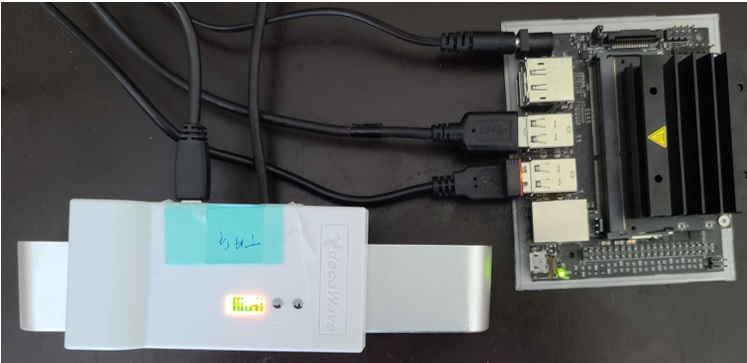
\includegraphics[width=1\linewidth]{fig/DWM_tag_setup.jpg}
\caption{DWM1001+Zed Camera interfacing with Jetson Nano.} \label{fig.structure}
\end{figure}

\subsubsection{Experimental Setup}
The ultra-wideband beacon DWM1001 can be configured into various modes such as tag, anchor, listener as mentioned in reference  [18].
\newline
Preparation of Anchors:

\begin{itemize}
\item Anchors are the unit that placed as a reference point at various locations in the indoor conditions.
\item Mount the anchors at the high level and within the line of sight as mentioned in Fig. 6.
\item Minimum 3  anchor units are required to establish an RTLS connection.
\item Power them using batteries or a power bank or a USB power adapter directly plugged to supply.
\end{itemize}

Preparation of Tag:

\begin{itemize}
\item A tag is the main unit deployed on the device whose location needs to be tracked in the inner conditions.
\item A minimum of 1 tag unit is required to establish a connection. Powering it is similar to anchor.
\end{itemize}

After powering up tag and anchors, we configure them using UART Shell Mode when DWM1001 is connected to Jetson Nano. The configuration steps are mentioned in Page 11[19] of the DWM1001 Deployment Guide.

\begin{figure}[htb]
\centering
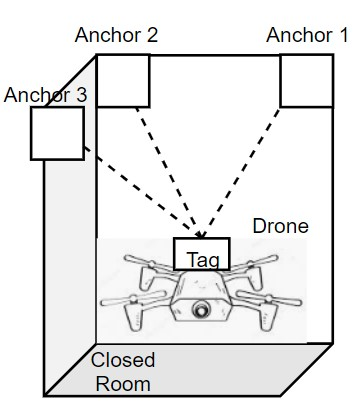
\includegraphics[width=0.5\linewidth]{fig/anchor_position_uwb.jpg}
\caption{DWM1001 tag and anchors placed inside a closed room.} \label{fig.structure}
\end{figure}

After configuring the tags and anchos, we place the anchors inside a closed room as shown in Fig. 4. The tag is connected to Jetson Nano(Drone). As per the DWM1001 instructions on page 28 of [18], we are positioning the anchors to establish the RTLS network.

\begin{figure}[htb]
\centering
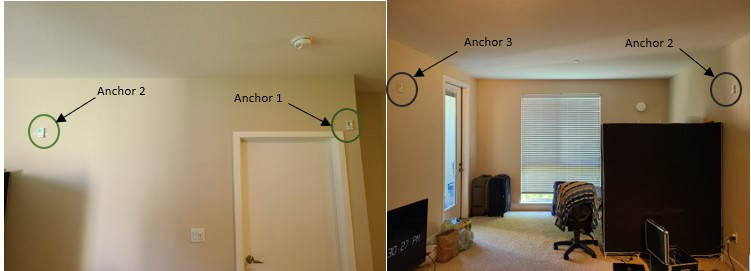
\includegraphics[width=1\linewidth,height=0.5\linewidth]{fig/anchor_position.jpg}
\caption{Actual anchor placement in indoor conditions.} \label{fig.structure}
\end{figure}

To evaluate the performance of DWM1001 in indoor conditions, we placed 3 DWM1001 at different corners of the room and configured them as the anchor as a part of an experimental setup as shown in Fig. 5 and Fig. 6. The DWM1001 along with the camera and drone is configured as a tag.

\begin{figure}[htb]
\centering
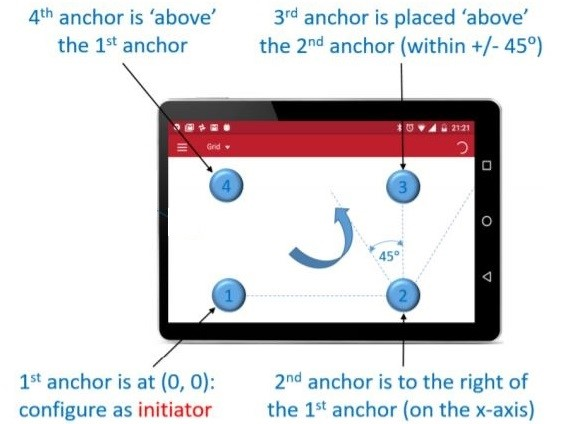
\includegraphics[width=\figwidthb]{fig/uwb_position_setup.jpg}
\caption{Anchor placement instructions.} \label{fig.structure}
\end{figure}

We evaluated the performance of the DWM1001 by comparing the values of (x,y,z) of the tag concerning the ground truth.

\subsubsection{Software Interface}
DWM1001 interacts with Jetson Nano over UART communication. We used UART shell mode to retrieve data from the tag. We have used a Python Script to parse the data from the string that is sent by DWM1001 to Nano. The following flow chart explains the step-by-step execution of our Python script. This python script is integrated with the depth-sensing component to achieve object tracking.

\begin{figure}[htb]
\centering
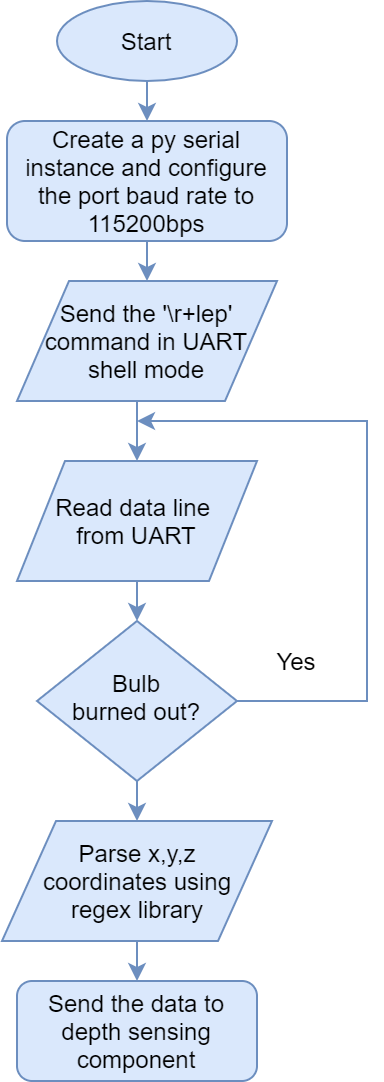
\includegraphics[width=0.42\linewidth]{fig/UWB_flow_diagram.png}
\caption{DWM1001 data parsing in Python.} \label{fig.structure}
\end{figure}

\subsection{Object Detection}

Object Detection is an integral part of our project. It enables the drone to detect obstacles in its path in real-time and avoid crashing into it enabling the drone to navigate along its path autonomously. Object detection finds wherein the frame various objects are located by extracting their bounding boxes. These bounding boxes indicate the objects in front of the drones which act obstacles in the pre-determined path of the drone.

\subsubsection{Jetson Nano and TensorRT}
The Jetson Nano Developer Kit has a Quad-core ARM A57 1.43 GHz and 128-core Maxwell architecture GPU. Nvidia provides its JetPack SDK which contains Linux OS and environments to build AI applications. The SDK supports NVIDIA TensorRT which enables high-performance deep learning inference. Application using TensorRT accelerates its performance by 40 times faster than CPU when real-time inference takes place. This allows optimizing Convolution Neural Nets (CNN) using many different deep learning frameworks, which can then be deployed to resource constraint embedded devices. TensorRT makes use of Nvidia’s CUDA platform to improve the inference for all major deep learning platform.[20]
\newline TensorRT scales down and quantizes the network parameter from FLOAT32 to INT8 and INT16 which reduces application latency required for many real-time embedded projects. The batch size parameter can be specified in the model which determines the number of images on which object detection is performed. Multiple layers like ReLU, Convolution, Bias of the model is optimized by fusing them to create a layer fusion. Also, layers that share the same input are fused which is called layer aggregation. Tensor RT also helps to run certain operations such as FlattenConcat which are not supported by Nvidia’s Runtime framework.

\begin{figure}[htb]
\centering
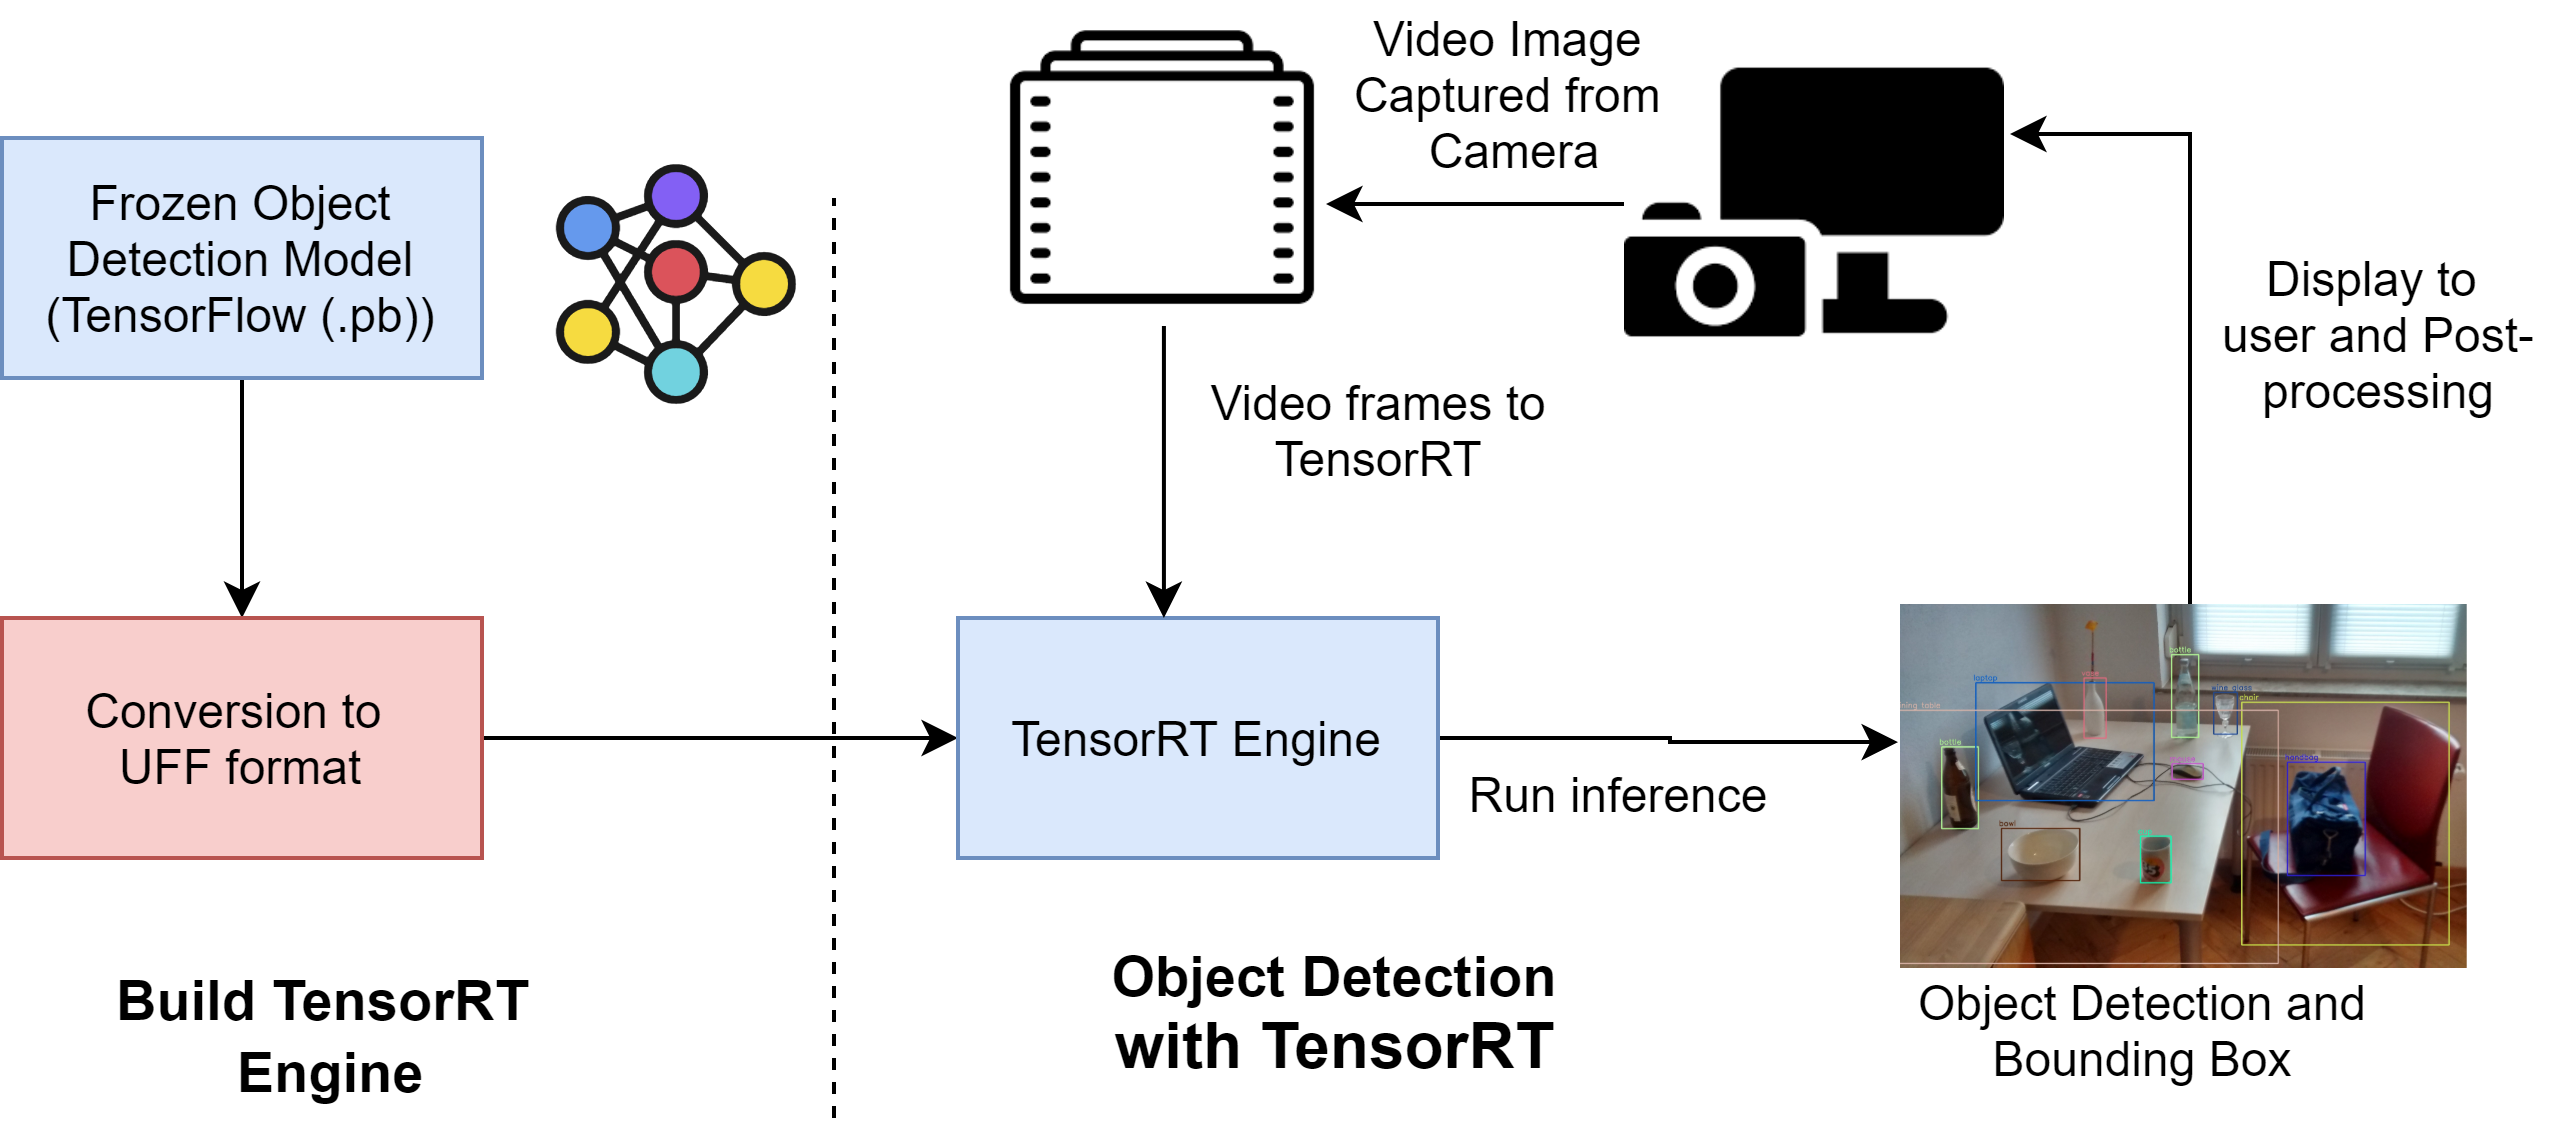
\includegraphics[width=1\linewidth]{fig/TensorRT_v2.png}
\caption{ TensorRT Workflow.} \label{fig.structure}
\end{figure}

In Fig 8, the entire workflow of the TensorRT and object detection is displayed. Any deep learning model in a framework such as TensorFlow, ONNX, PyTorch can be obtained. The frozen graph of the model (here TensorFlow model is depicted) is passed on the TensorRT build engine. The TensorRT build engine converts the model into Universal Frame Format (UFF). The engine then applies optimizations to the model such that it can take advantage of GPU based hardware and accelerate the performance and inference. The model can now detect the GPU and run code automatically using the GPU’s tensor core. Appropriate memory size is provided to the model by the engine to perform and store the intermediate computations. A camera connected to the Jetson Nano captures live video images from the surrounding environment. The TensorRT engine receives image frames from the captured video. It then performs pre-processing to the image such as shifting the order of the axis, normalizing, and flattening the image for faster inferencing. A timer is used to measure the time taken for performing inference on the captured image. After performing the inference for object detection, the TensorRT engine will return the arrays consisting of bounding boxes for the located object, the confidence level for each object in the image, and the class to which the detected object belongs to. Finally, these arrays are used to overlay the image capture with the information about coordinates, confidence level, and class to the user. The user can take appropriate action.

\subsubsection{Model Selection for Object Detection}
The main requirement for selecting a model for object detection for speed and accuracy. The model to be selected should have minimum latency since object detection and avoidance should have to perform in real-time. The model should also be accurate enough to make the correct object detection. Unfortunately, the Jetson Nano development board has limited resources and computation power. Thus, selecting the model for object detection a tradeoff had to be made between speed and accuracy of the model. The model under consideration for selection is SSD-Mobilenet-v2 and Yolov3 which are optimized using Nvidia’s TensorRT. After evaluating the performance of both models, we concluded that SSD-Mobilenet-v2 is more accurate but slower than the Yolov3 model. Since accuracy is a priority for object detection, we decided to use the SSD-Mobilenet-v2 model for object detection in our application. The model is trained using the MS COCO dataset which contains 330,000 images of 91 different classes such a person, chairs, cars, planes, water bottles, laptops, desk, etc. 

\subsection{Depth Sensing}
The ZED camera is a stereo camera i.e. it has two cameras separated by a certain distance called the baseline. This true for the human eyes which can perceive depth because of the distance between them and we try to mimic it. If the baseline is small, the depth perception for objects close to the camera would be excellent, but it would be inaccurate for faraway objects. If we keep on increasing the baseline, we could accurately measure the length of the faraway objects (given a camera with good quality image capturing ability) but the minimum distance for capturing the depth information would increase. This happens because the left and right images will capture an object at different positions due to the baseline separation i.e. there would be a shift in pixels. The depth is inversely proportional to the shift in the pixels. Thus, closer objects would appear more shifted and the faraway objects would appear less shifted between the left and right images.

\begin{figure}[htb]
\centerline{\subfloat{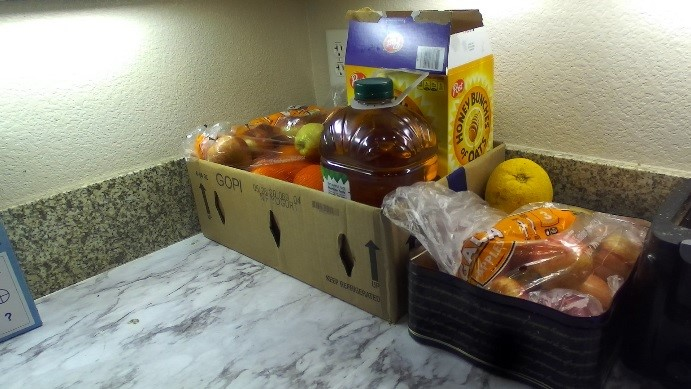
\includegraphics[width
=0.5\linewidth]{fig/left_img.jpg}} \hfil
\subfloat{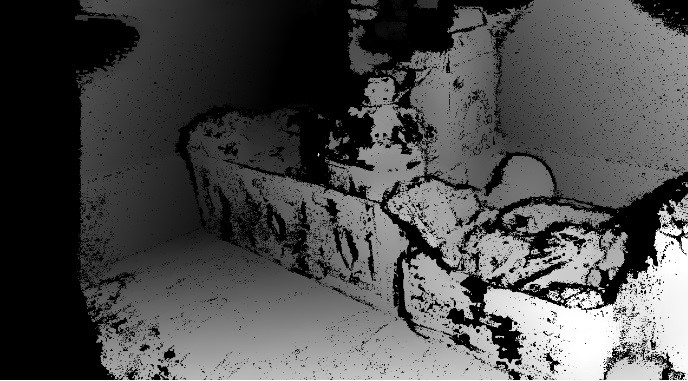
\includegraphics[width=0.5\linewidth]{fig/depth_img.jpg}}
} \caption{(a) Left camera image; (b) Depth map after processing the left and right image.} \label{fig.doublefigure}
\end{figure}

\begin{figure}[htb]
\centering
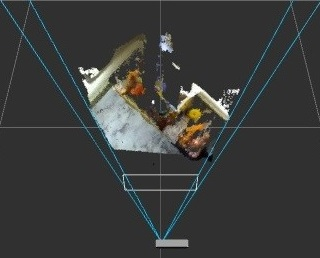
\includegraphics[width=\figwidthb]{fig/bird_eye}
\caption{ Bird Eye view from the point cloud data.} \label{fig.structure}
\end{figure}

The ZED camera SDK has many API’s for python and C++ to control the camera and get the depth and point cloud. We make use of the python for building our application. It uses the above-discussed techniques to obtain the depth information in an image. We make use of the ZED SDK as it utilizes CUDA and Nvidia GPU to parallelize the processes like block matching, getting depth map from disparity, etc.
After retrieving the depth mode, we construct the 3D point cloud. This helps us to get the distance to a pixel by using the Euclidean distance formula:

\[distance_{x,y} = \sqrt{x^{2}+y^{2}+z^{2}}\]

Fig 9(a). shows the left image which is combined with the right image to get a disparity map. Based on the disparity we calculate the depth of each pixel. A depth map is shown in Fig 9(b). We can access the depth values using the camera coordinates. Now, based on the image coordinates (x, y, z) and intrinsic cameras sensor parameters such as focal length (fx, fy) and optical center coordinates (cx, cy) we can get the world coordinates for the objects w.r.t. the camera. We can get the parameters fx, fy, cx, and cy directly from the ZED camera calibration file. We can see the bird-eye view of the point cloud in Fig. 10 which has the real world coordinates plotted based on camera as origin. The formula for getting world coordinates is:

\[X = \frac{depth}{fx*(x-cx)}\]
\[Y = \frac{depth}{fy*(x-cy)}\]
\[Z = depth_{x,y}\]

From the above equations, assuming that the camera is at location (0, 0, 0) i.e. the origin, we can calculate the objects location (X, Y, Z). The flow diagram for accessing the object coordinates is shown in Fig. 11.

\begin{figure}[htb]
\centering
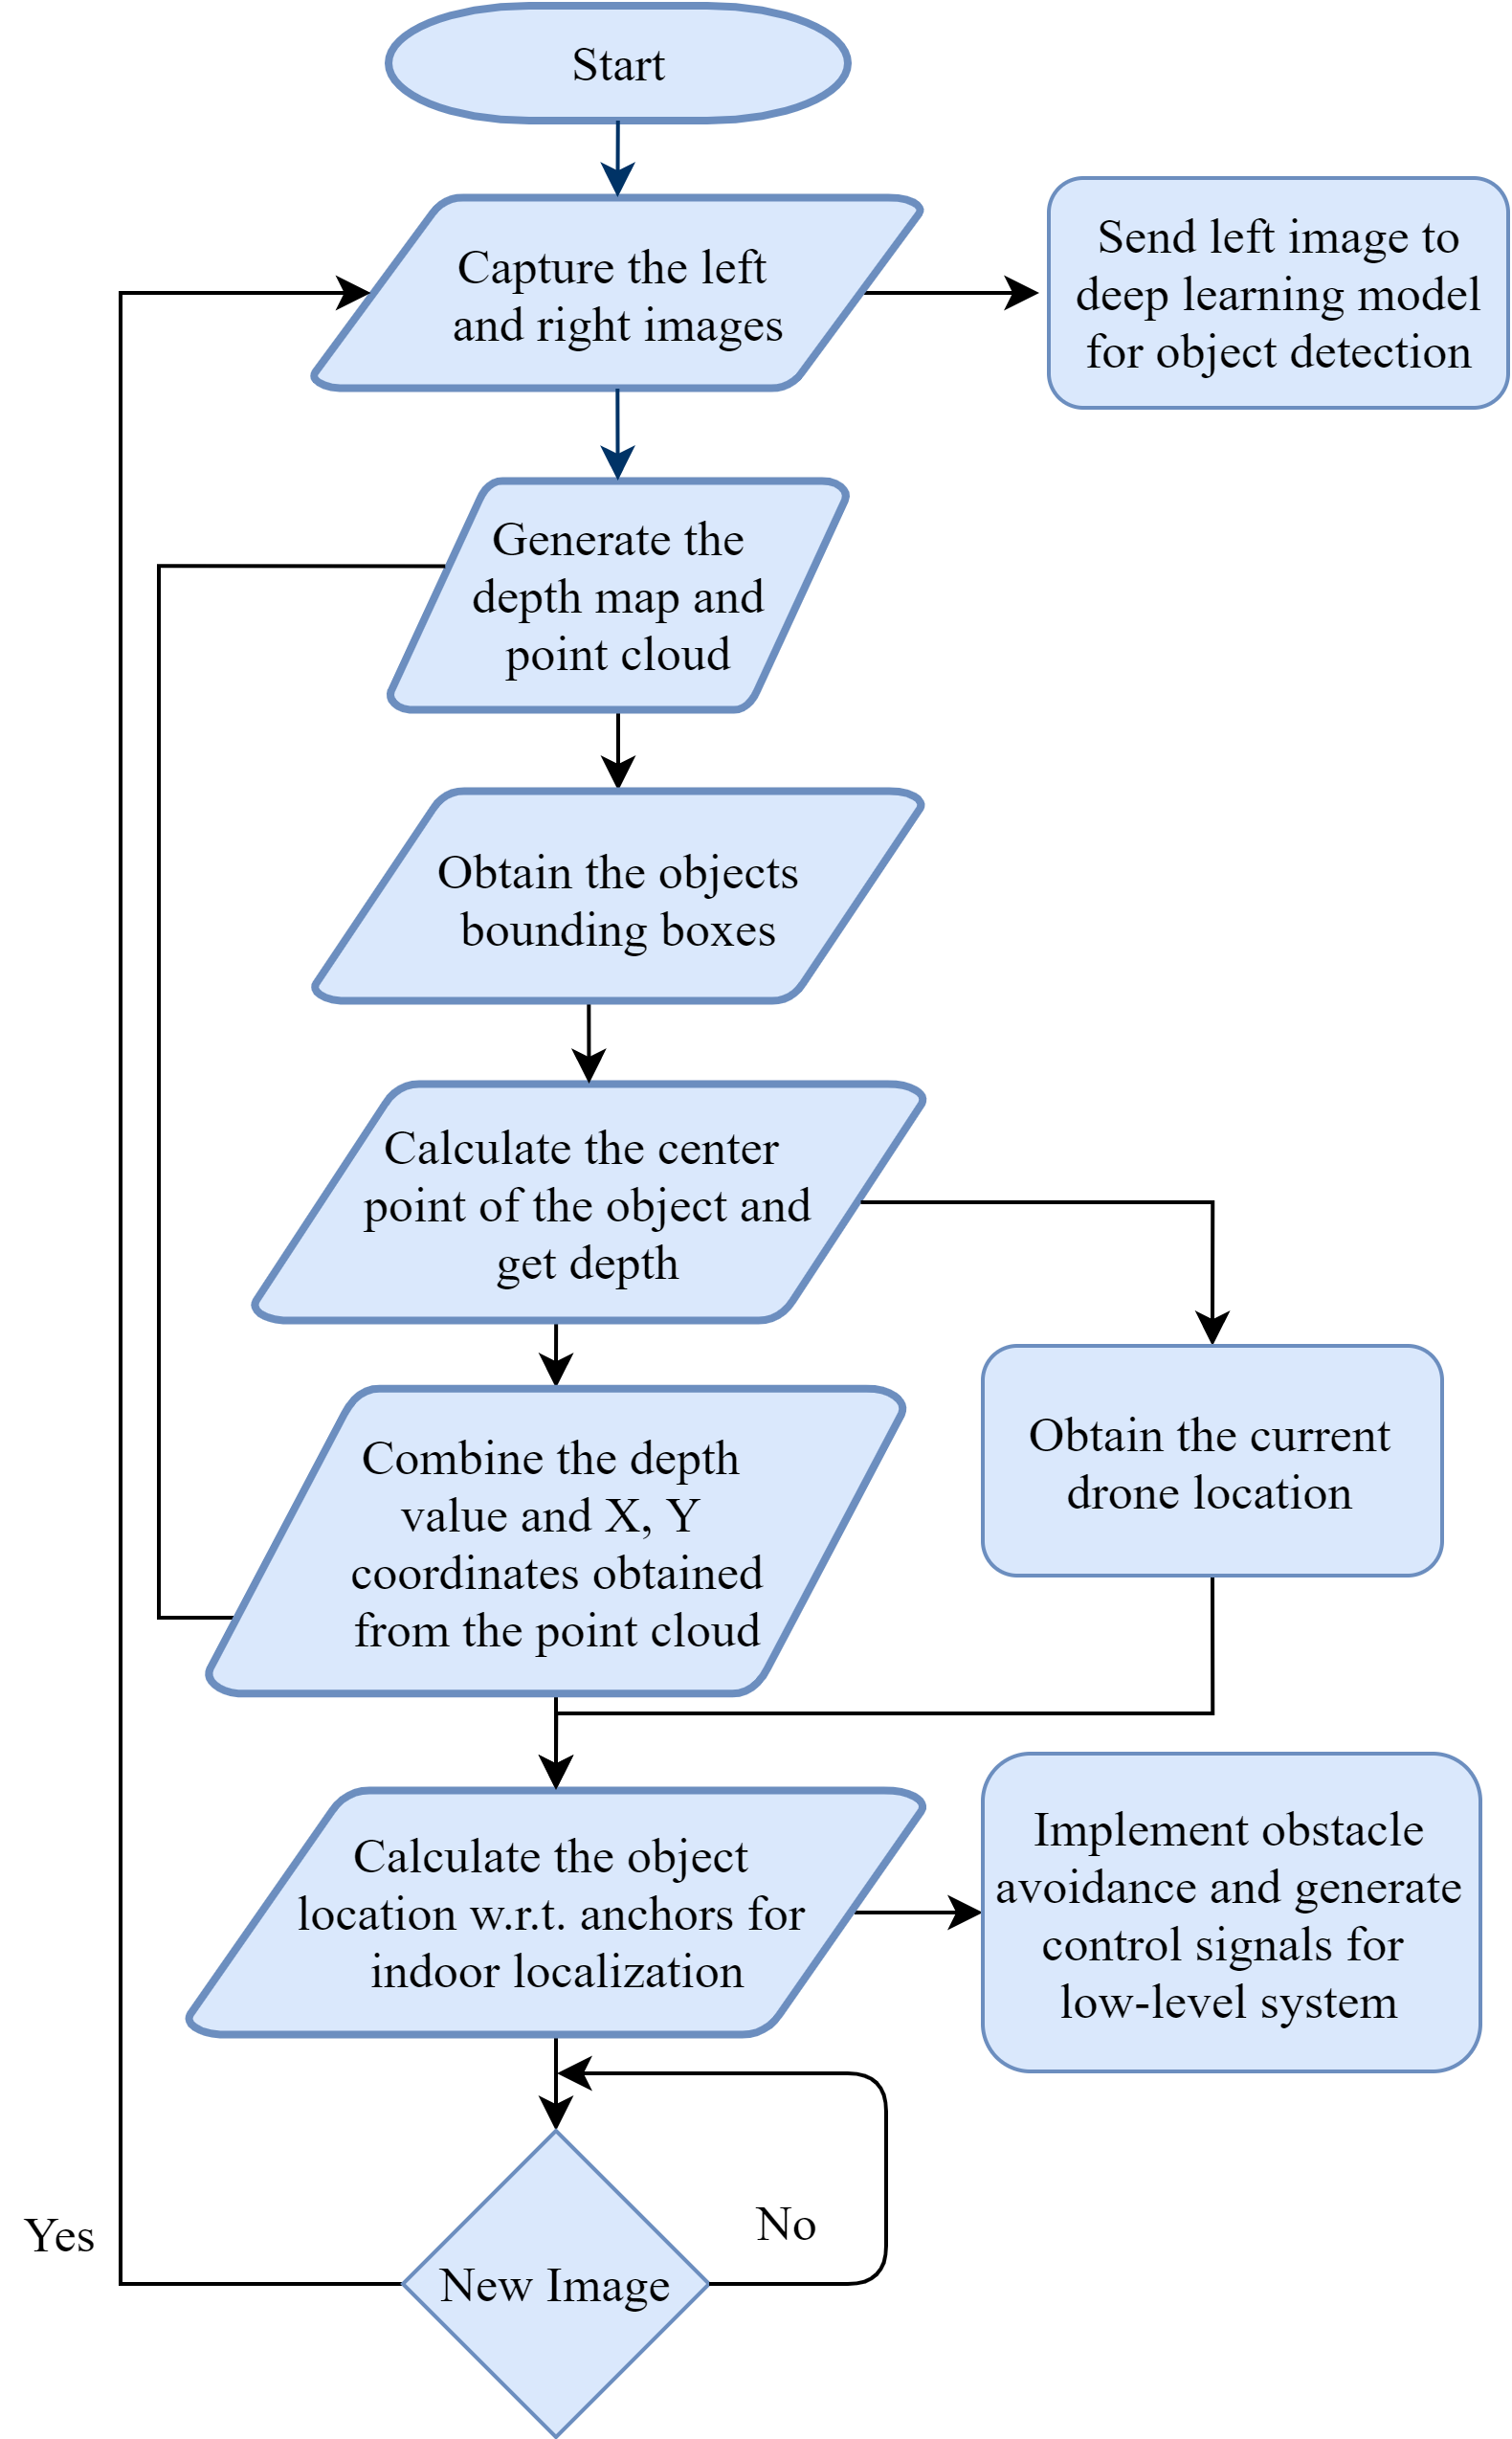
\includegraphics[width=0.9\linewidth]{fig/flow_depth_sensing.png}
\caption{Depth Sensing flow diagram.} \label{fig.structure}
\end{figure}


\section{Evaluation Methodology and Results}\label{sec:evaluation}

\subsection{UWB Localization}
During the experimental setup, we placed anchors at different locations inside the room and measured the coordinates. The  coordinates of Anchor1 is (0,0,0), Anchor 2 is (3.61,0,0) and Anchor 3 is (3.8,3.61,0). Here, Anchor 1 acts as an initiator(origin) and the measurement unit is in meters. 
\newline We also evaluated the values of (x,y,z) of tag at different positions inside the closed room and measured the corresponding ground truth and analyzed the data in excel by calculating the percent error parameter. Below is the graph showing the comparative analysis of DWM1001 coordinate values versus the actual ground truth values. We also computed the Euclidian distance of tag to Anchor 1 and evaluated the variations to calculate the percentage error.

\begin{figure}[htb]
\centering
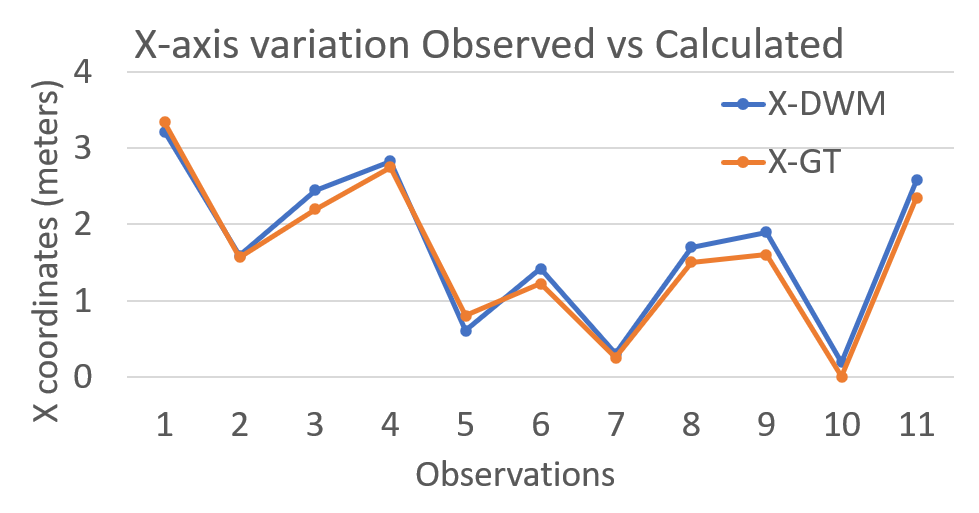
\includegraphics[width=1\linewidth]{fig/uwb_x_graph.png}

\centering
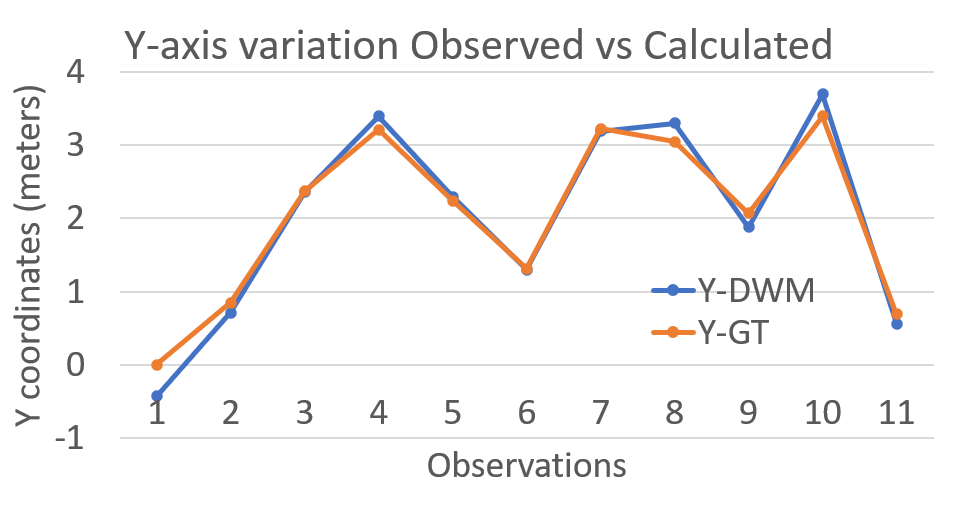
\includegraphics[width=1\linewidth]{fig/uwb_y_graph.png}

\centering
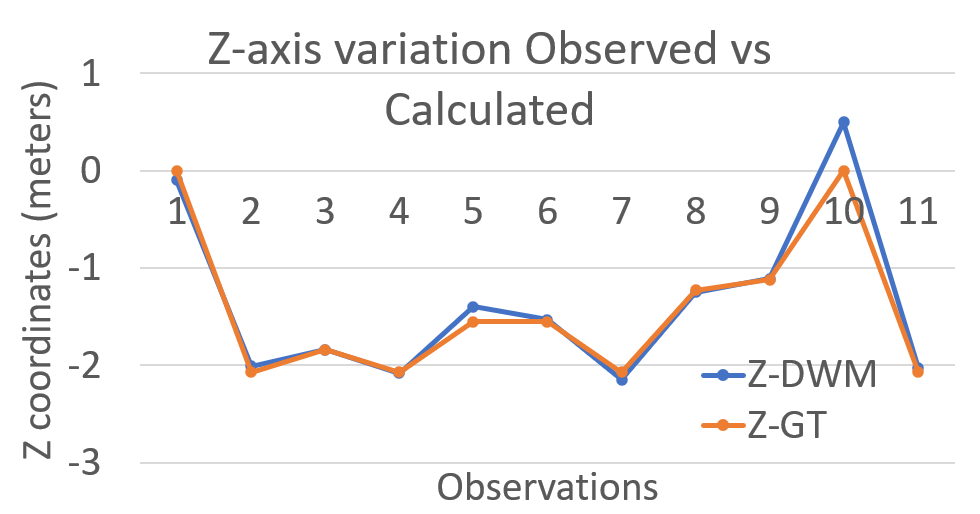
\includegraphics[width=1\linewidth]{fig/uwb_z_graph.png}
\caption{Variations of DWM1001 tag (X, Y, Z) coordinates concerning ground truth.} \label{fig.structure}
\end{figure}

\begin{figure}[htb]
\centering
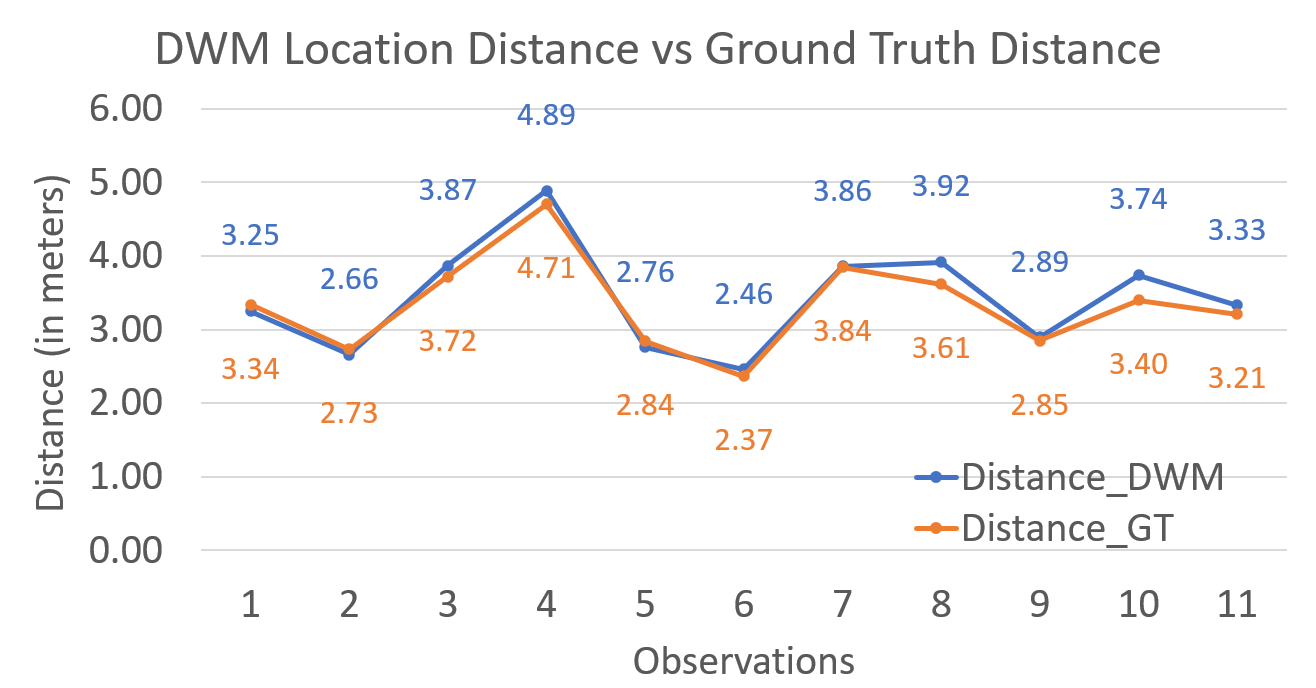
\includegraphics[width=1\linewidth]{fig/uwb_distance_graph.png}
\caption{DWM1001 location distance vs ground truth (in meters).} \label{fig.structure}
\end{figure}

The accuracy of the DWM1001 distances measured relative to the anchors was around 96 percent with a percentage error of 4.06{\%}. We also evaluated the variations of x y and z and calculated the average percentage errors. The percentage error for x,y,z came out to be 11.16{\%}, 6.6{\%}, and 2.1{\%} respectively. 
In summary, we were able to achieve the maximum error of ±0.41m for the x-axis, ±0.25m for the y-axis, and ±0.04m for z-axis movements of the DWM1001 tag attached to Jetson Nano.

\subsection{Model Selection for Object Detection}
The main requirement for selecting a model for object detection for speed and accuracy. The model to be selected should have minimum latency since object detection and avoidance should have to perform in real-time. The model should also be accurate enough to make the correct object detection. Unfortunately, the Jetson Nano development board has limited resources and computation power. Thus, when selecting the model for object detection a tradeoff had to be made between speed and accuracy of the model. The models under consideration are SSD-Mobilenet-v2 Tiny Yolov3 and SSD-RESNET-18. These models are based on the TensorFlow framework. The models which are in the graph format are converted to network objects.

\begin{figure}[htb]
\centering
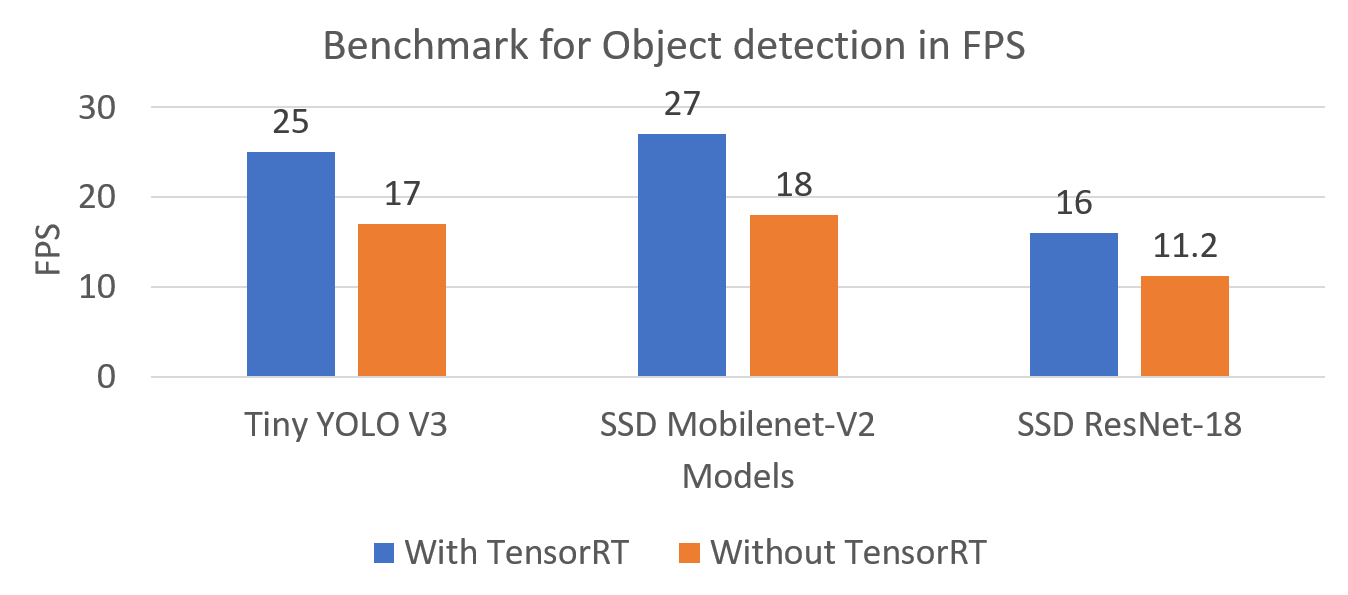
\includegraphics[width=\figwidthb]{fig/benchmark.png}
\caption{Performance benchmark of different Object Detection Models.} \label{fig.structure}
\end{figure}

\begin{figure}[htb]
\centering
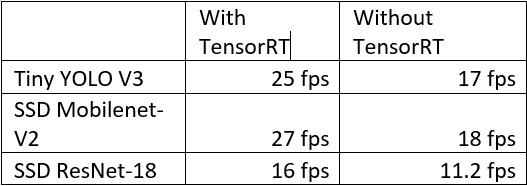
\includegraphics[width=\figwidthb]{fig/Table.jpg}
\caption{Table for benchmark.} \label{fig.structure}
\end{figure}

To determine the improvement in performance achieved using optimizing the network through TensorRT, the object detection models are compared. As per the figures, models not optimized using TensorRT are 30 percent slower than models optimized using TensorRT. This is a significant performance gain. Also, the SSD-Mobilenet-v2 models have a maximum inference speed due to the higher frame rate per second. Since SSD-Mobilenet-v2 has a better performance compared to Tiny Yolov3 and SSD-RESNET-18 model we chose the SSD-Mobilenet-v2 model for object detection in our application. The model is trained using the MS COCO dataset which contains 330,000 images of 91 different classes such a person, chairs, cars, planes, water bottles, laptops, desk, etc.

\subsection{Obstacle Detection using Camera}
To evaluate the object detection model on the Jetson Nano initially a pre-trained SSD-Mobilenet-v2 is passed an input image consisting of multiple persons.

\begin{figure}[htb]
\centering
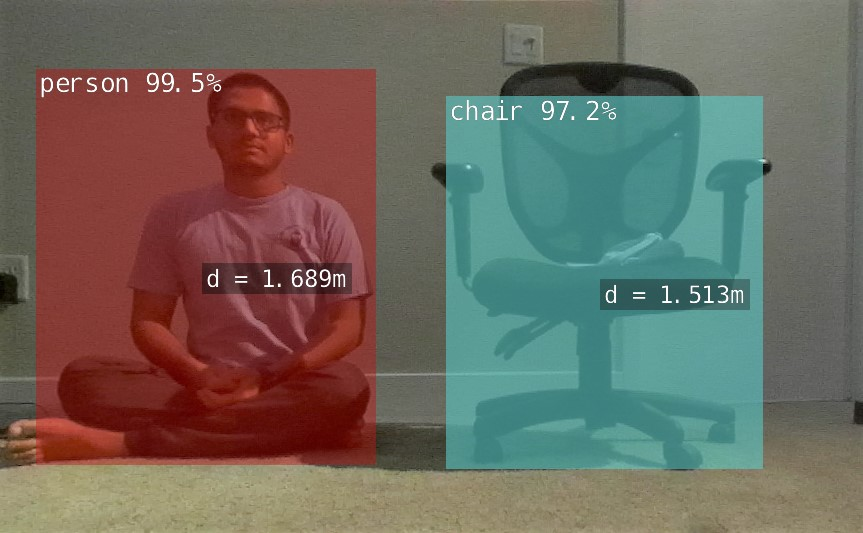
\includegraphics[width=\figwidthb]{fig/obj_detect_saumil.jpg}
\caption{Object Detection flow diagram.} \label{fig.structure}
\end{figure}

Once the pre-trained object detection model is tested against sample input images, an application of object detection for a drone is created by inferencing on real-time captured images. We can see the flowchart below

\begin{figure}[htb]
\centering
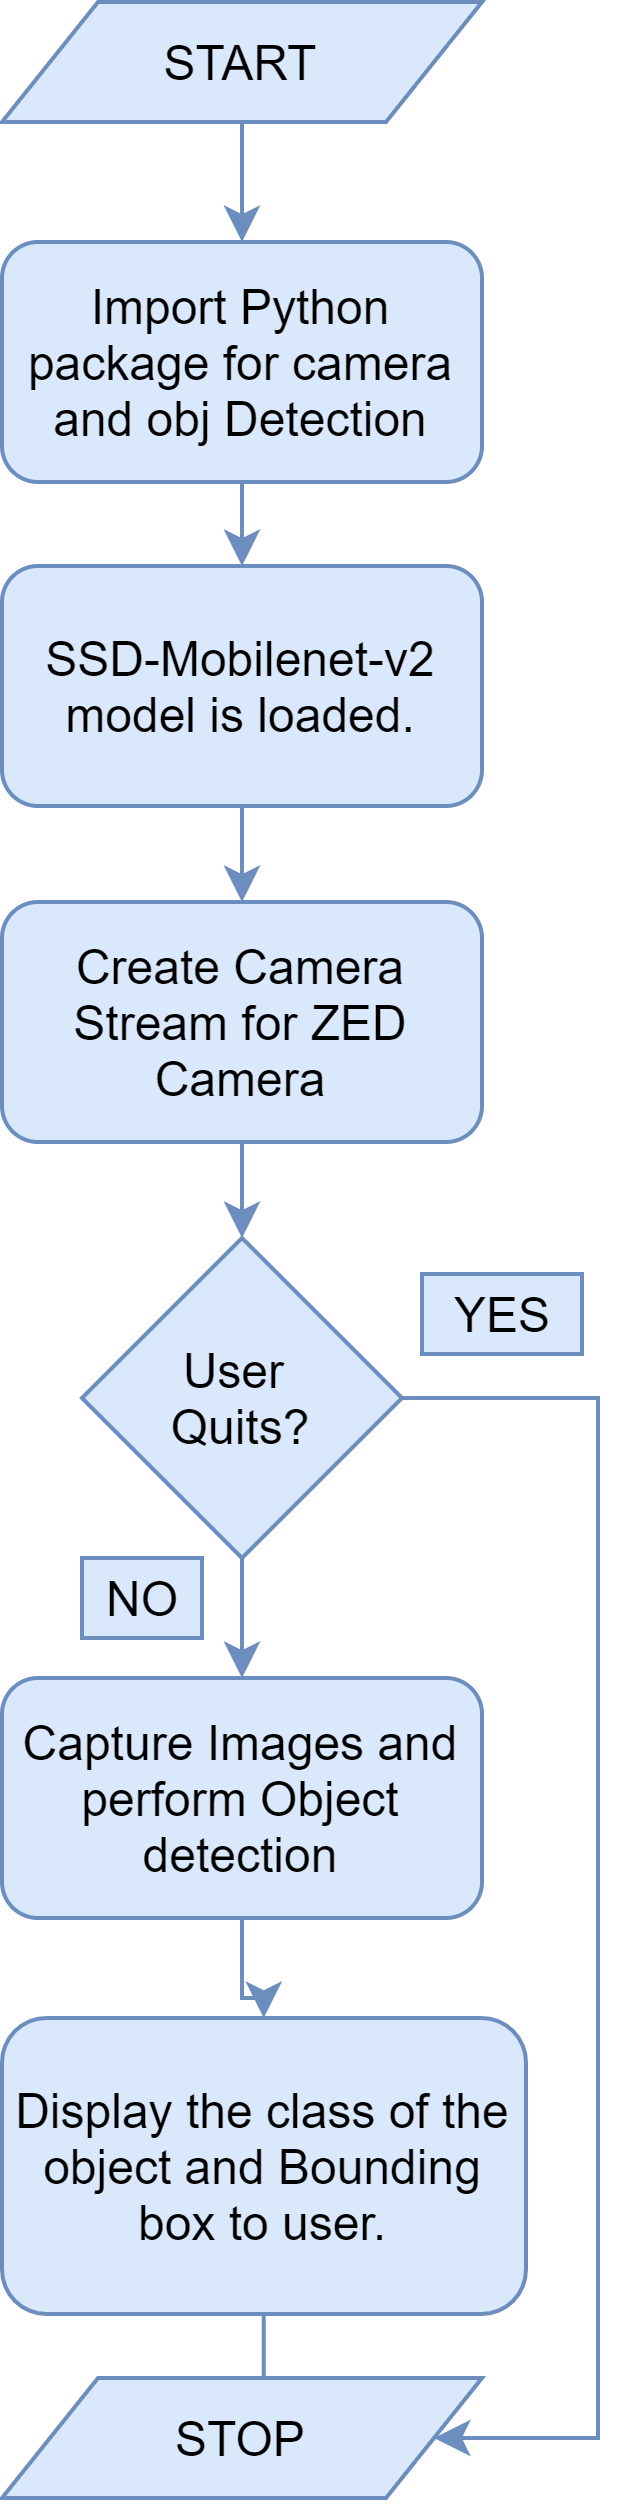
\includegraphics[width=0.4\linewidth]{fig/flow_saumil.png}
\caption{Object Detection.} \label{fig.structure}
\end{figure}


\subsection{Depth sensing using Stereo Camera}
We made use of the ZED camera to capture the depth of the obstacles which are in the front of the drone. First, the obstacle detection model was run on the image obtained from the ZED. Based on the objects detected, we retrieve the depth on that object which can be seen in Fig 6. The output of the code is shown in Fig. 18 which shows the objects, their name and the distance to the object from the camera.

\begin{figure}[htb]
\centering
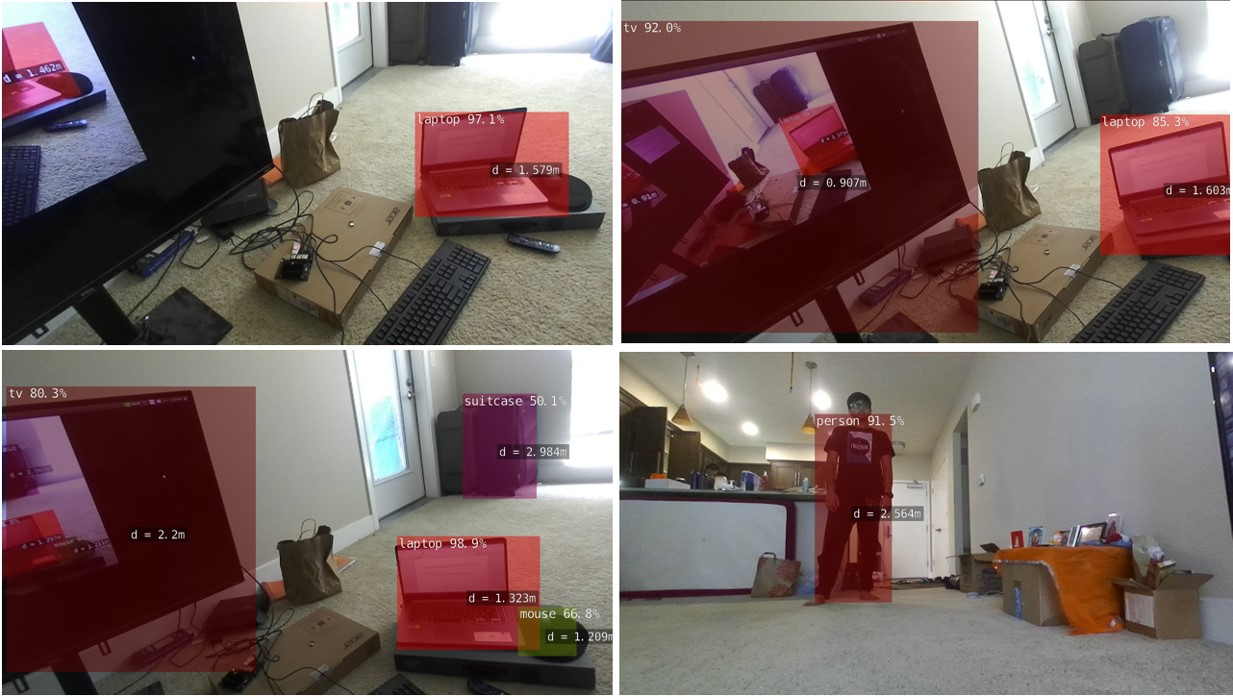
\includegraphics[width=1\linewidth]{fig/depth_jay.jpg}
\caption{Depth Detection.} \label{fig.structure}
\end{figure}

After retrieving the depth of all the objects in the image, we did some experiments for evaluating the accuracy of our depth sensing module. We kept the camera at a stationary position and calculated the depth and distance of the various object that was detected in the image. Simultaneously, we collected the ground truth values for the objects as well. The ground truth depth values were measured physically using the measuring tape. To calculate the accuracy, we plotted the results i.e. calculated depth vs ground truth depth and obtained the results shown in Fig. 19

\begin{figure}[htb]
\centering
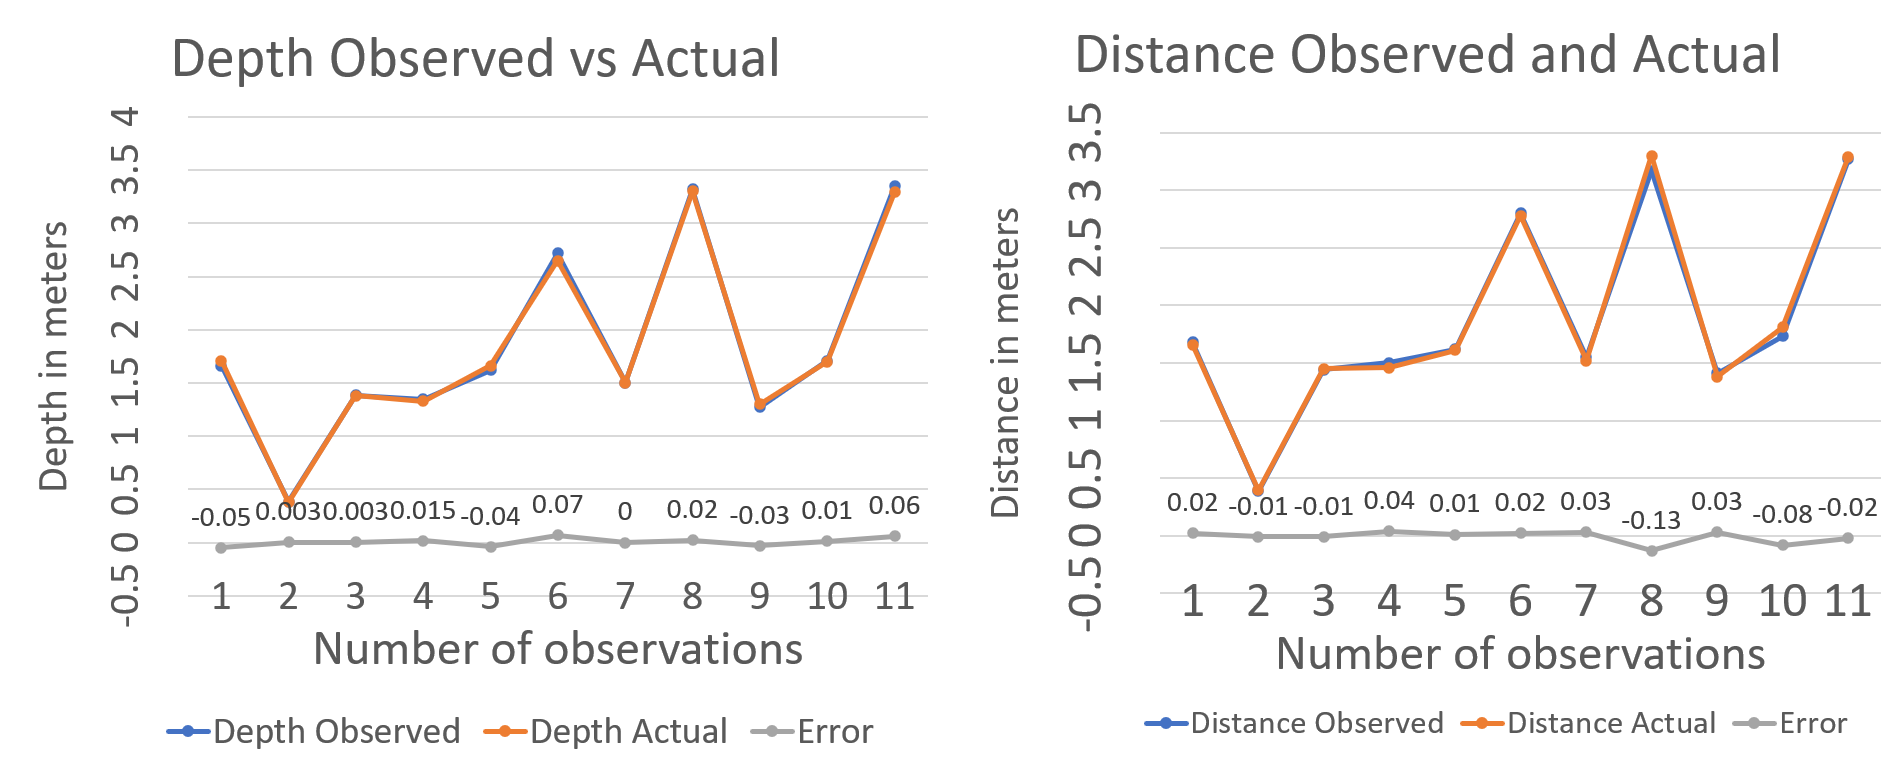
\includegraphics[width=1\linewidth]{fig/jay_graph.png}
\caption{Graph for depth and distance detection.} \label{fig.structure}
\end{figure}

As we can see that the error in detecting the depth and distance of the object is very minimal. For depth, the maximum error is ±0.07 meters and maximum error for measuring the distance is ±0.13 meters over a range of about 4 meters. Thus, if we calculate the error rate that would be about 1.75{\%} for depth and 3.01{\%} for distance. This suggests that the depth-sensing result for the objects is quite accurate. The observed frame rate that we obtained for the entire process after object detection and distance measurement was about 10 to 15 FPS. The drop in the frame rate resulted due plotting multiple bounding boxes in the image and converting the ZED image frame to the CUDA capsule resulting in multiple steps.

\subsection{Integrating high-level components}
We assessed the accuracy and error rate for the high-level components composed of object detection, depth sensing, and ultrawideband beacon individually. The target for our high-level system was to obtain the (X, Y, Z) coordinates of the objects that were in the path of our drone to avoid them. Thus, after integrating the object detection, depth sensing, and ultrawideband beacon, we were able to obtain the object localization. The UWB module is placed on the drone with the camera. So, based on the UWB results we get the current location of the drone in the indoor environment w.r.t the 3 anchors placed inside the room. The set up for this is shown in Fig. 20. We match the coordinate system of the UWB module and ZED camera as shown in Fig. 21.

\begin{figure}[htb]
\centering
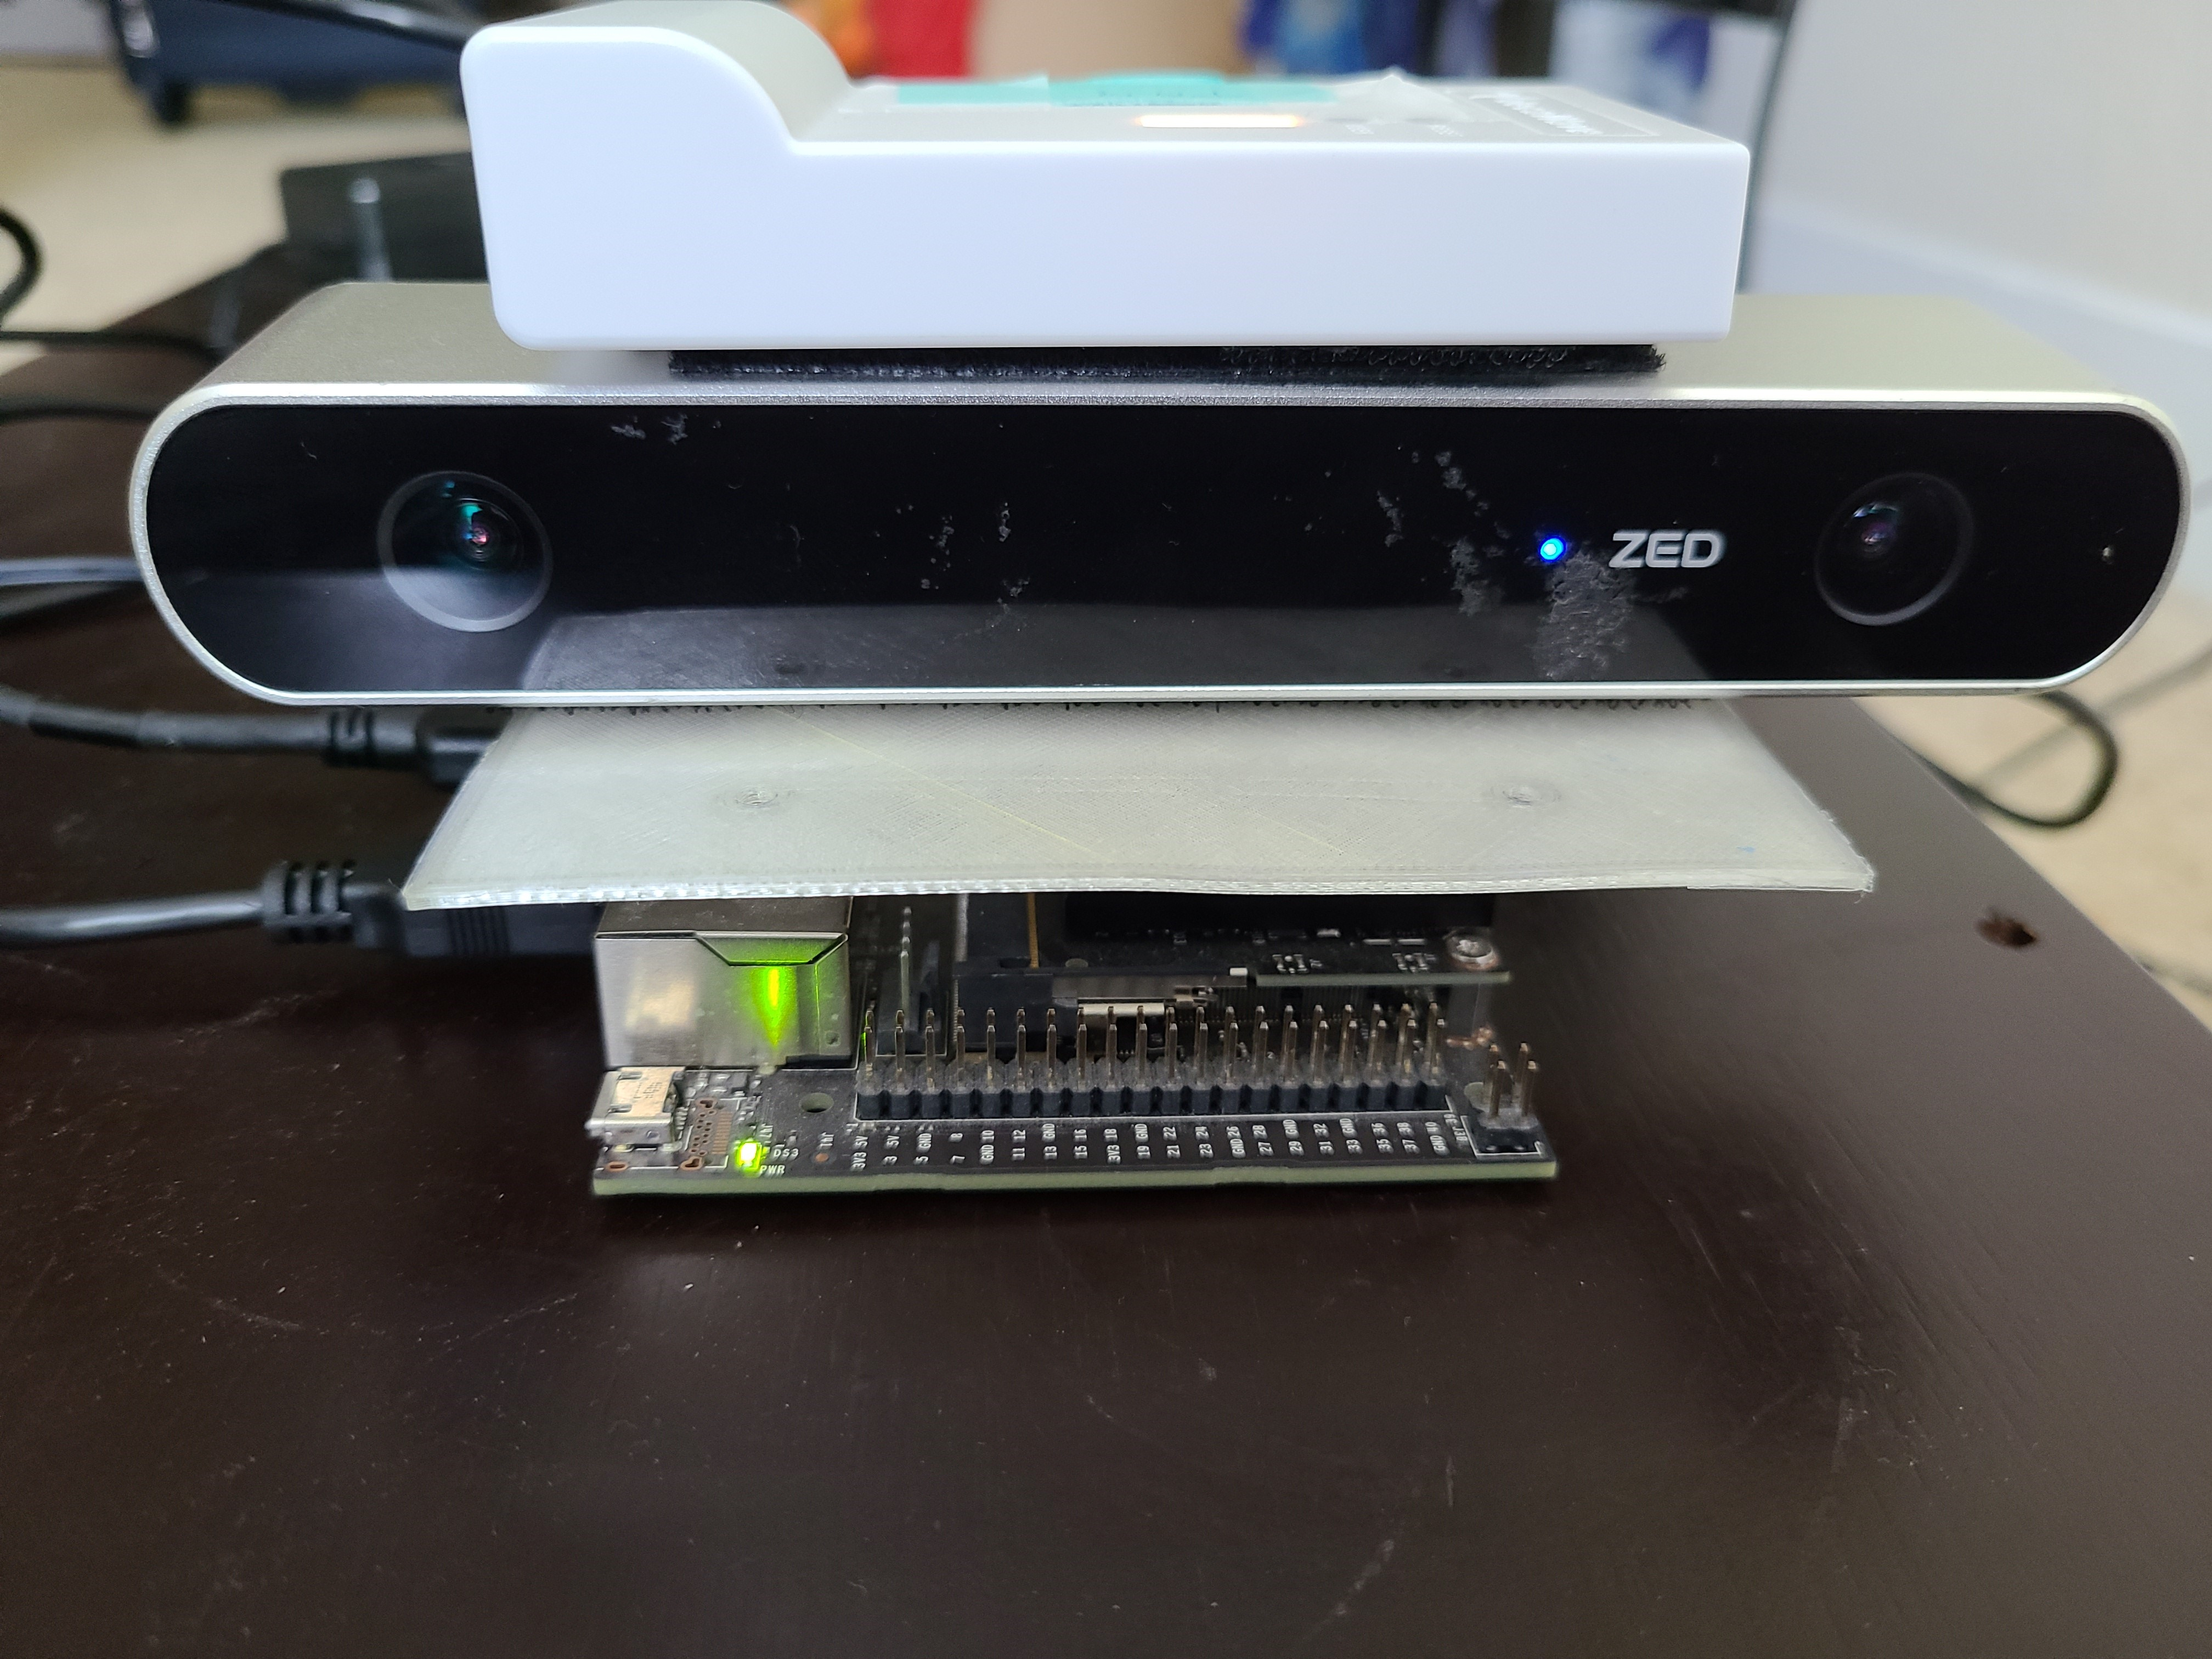
\includegraphics[width=0.7\linewidth]{fig/zed_setup_jay.jpg}
\caption{Camera Setup.} \label{fig.structure}
\end{figure}

\begin{figure}[htb]
\centering
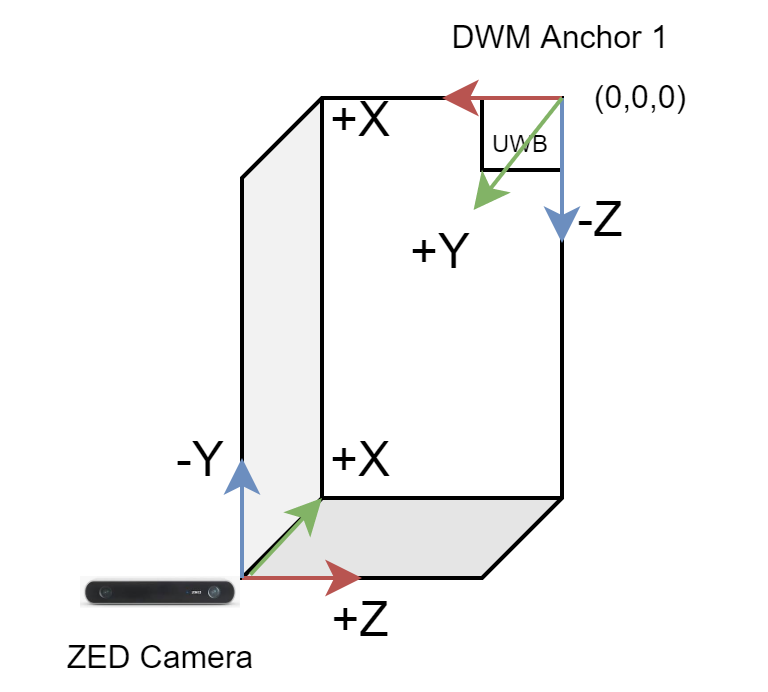
\includegraphics[width=0.5\linewidth]{fig/coordinate_matching.png}
\caption{Coordinate system matching of the UWB module and ZED camera for our setup.} \label{fig.structure}
\end{figure}

We then obtain the bounding boxes from the detected objects. This information is useful for extracting the objects’ camera-based coordinates, which are then converted to real-world coordinates. The camera is at position (0, 0, 0), and based on camera as origin we get the objects real-world coordinates. We obtained the object localization as we can see in Fig. 22.

\begin{figure}[htb]
\centering
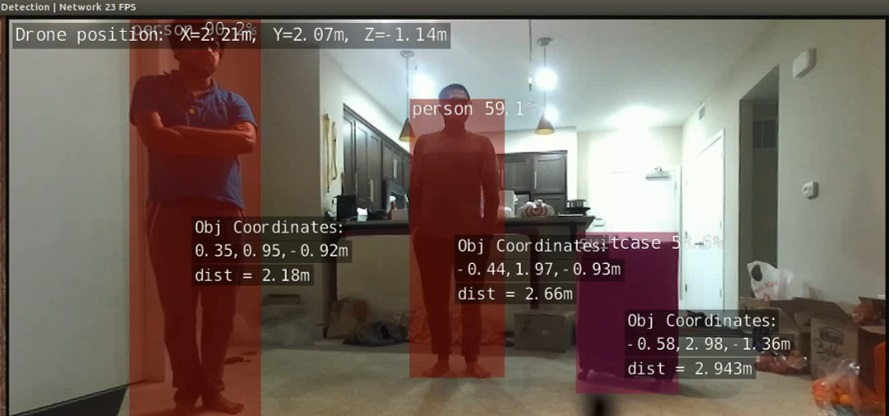
\includegraphics[width=1\linewidth]{fig/final_detect_jay.jpg}
\caption{Final object localization.} \label{fig.structure}
\end{figure}

For evaluating the accuracy of object localization, we conduct some experiments. We measure the ground truth results with the calculated results and take 10 observations. The camera was at a fixed position and the object was moved around inside the room. So, we traced the path and visualized the error after plotting it as shown in Fig. 24.

We now go into the details of the experiment step-by-step. The first task was to detect all the objects in the image and get the bounding boxes from the machine learning model.

\lstset{language=Python}
\lstset{label={lst:code_direct}}
\lstset{basicstyle=\footnotesize}

\begin{lstlisting}
bounding_boxes = net.Detect(left_image_from_camera, 
			   image_width, image_height)
\end{lstlisting}

After getting the bounding boxes we get the center of all the objects in the image. We retrieve the point cloud i.e. (X, Y, Z) real-world coordinates for every pixel in the image as shown in Fig. 10. The pixel (X, Y, Z) coordinate will be w.r.t camera (0, 0, 0).

\begin{lstlisting}
zed.retrieve_measure(point_cloud, sl.MEASURE.XYZRGBA)
\end{lstlisting}

The center of the object will be useful in extracting their real-world coordinates direclty from the computed point cloud. The concept is shown in Fig. 23

\begin{lstlisting}
camera_to_object_x_y_z = point_cloud.get_value(
			center_of_object_in_image_x, 
			center_of_object_in_image_y
			)
\end{lstlisting}

\begin{figure}[htb]
\centering
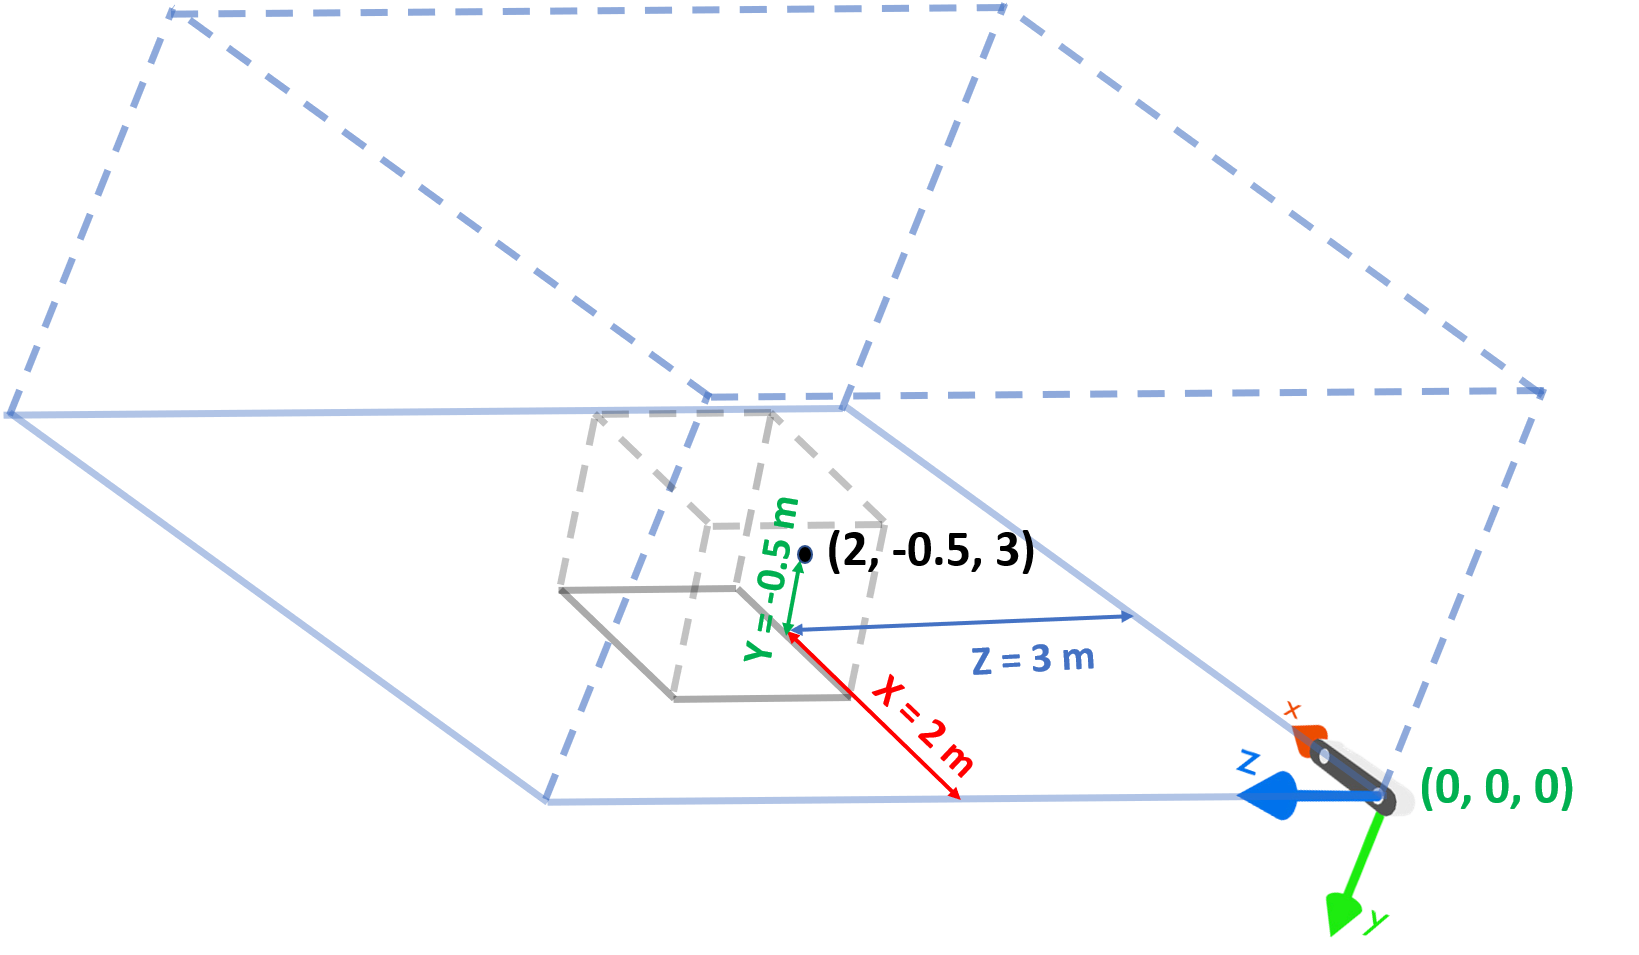
\includegraphics[width=0.85\linewidth]{fig/camera_to_obj_world.png}
\caption{Object coordinates with camera as origin.} \label{fig.structure}
\end{figure}
Now, we need the object coordinates w.r.t the Anchor 1 to perform localization. So, we get the camera coordinates mounted with tag from the Anchors placed in the room and add/subtract the actual camera coordinates available from DWM to the location of the object available from the camera.

\begin{lstlisting}
dwm_to_object_x = (dwm_to_camera_x - 
		  drone_to_object_x)
dwm_to_object_y = (dwm_to_camera_y + 
		  drone_to_object_y) 
dwm_to_object_z = (dwm_to_camera_z - 
		  drone_to_object_x)
\end{lstlisting}

Through our calculations shown above, we get the object (X, Y, Z) as (-0.44, 2.1, -1.11) w.r.t DWM module i.e. we achieve object localization.

\begin{figure}[htb]
\centering
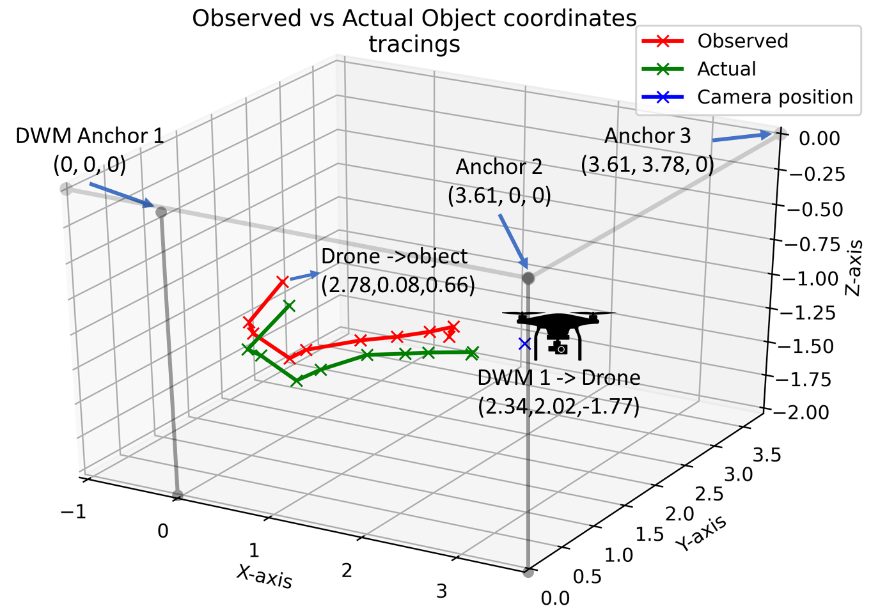
\includegraphics[width=1\linewidth]{fig/room2.png}
\caption{Object Localization environment for the experimental setup and observations. DWM at (0,0,0), drone position (2.34,2.02,-1.77) w.r.t DWM , and object position (2.78,0.08,0.66) w.r.t drone/camera.} \label{fig.structure}
\end{figure}

The 3D plot in Fig. 24 mimics the actual set up that we used for evaluation. The 3 anchors and drone attached with tag (blue ‘x’ mark) were placed with the coordinates shown. The calculated coordinates are shown with the red line and the ground truth is shown with a green line. As we can see the error between them is less. To visualize the error more prominently, we calculated the Euclidean distance and plotted them in Fig. 25. We can see that the ground-truth line and the calculated line match very closely in the graph based on the objects location.

\begin{figure}[htb]
\centering
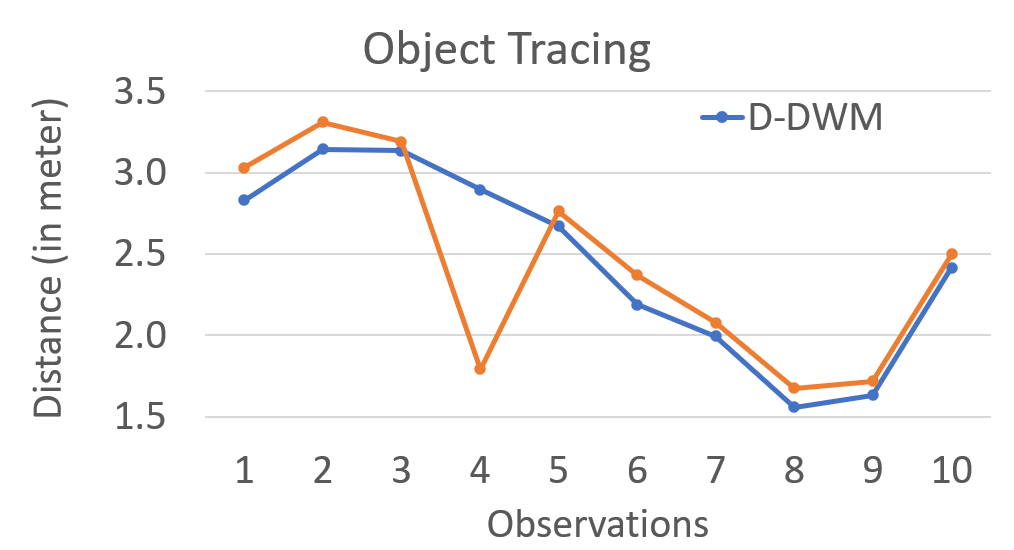
\includegraphics[width=1\linewidth]{fig/error_graph_obj_local.png}
\caption{Ground truth distance vs calculated distance.} \label{fig.structure}
\end{figure}

\begin{figure}[htb]
\centering
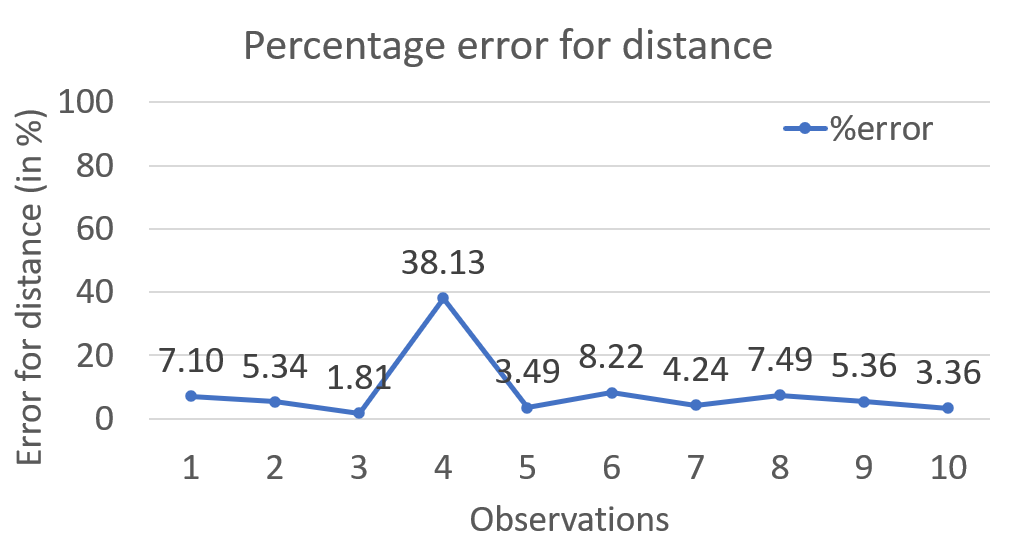
\includegraphics[width=1\linewidth]{fig/error_trace_percent.png}
\caption{Distance error rate for the experimental setup.} \label{fig.structure}
\end{figure}

To emphasize the accuracy, we calculated the error percentages for the difference in the Euclidean distance for each observation and plotted it as shown in Fig. 26. The error rate is well in the range of 1.81{\%} to 8.45{\%}. The average error rate for the 10 observations comes out to be 8.45{\%}.


\section{Conclusions}\label{sec:conclusions}
In this paper, we have presented a connected and autonomous robotic system that integrates multiple sensors for obstacle detection, depth perception, and UWB localization. We were able to achieve indoor localization using UWB with the error rate of 4.06 percent. For object detection, we selected SSD MobileNet v2 model whose performance was optimized using TensorRT. This project also demonstrated object tracking using depth sensing via ZED Camera 9with the measured localization error rate of 8.5 percent with respect to ground truth. This application of this project are surveillance of indoor environment and disaster relief.


% conference papers do not normally have an appendix

%The authors would like to thank...

% trigger a \newpage just before the given reference
% number - used to balance the columns on the last page
% adjust value as needed - may need to be readjusted if
% the document is modified later
%\IEEEtriggeratref{8}
% The "triggered" command can be changed if desired:
%\IEEEtriggercmd{\enlargethispage{-5in}}

% references section

% can use a bibliography generated by BibTeX as a .bbl file
% BibTeX documentation can be easily obtained at:
% http://mirror.ctan.org/biblio/bibtex/contrib/doc/
% The IEEEtran BibTeX style support page is at:
% http://www.michaelshell.org/tex/ieeetran/bibtex/
%\bibliographystyle{IEEEtran}
% argument is your BibTeX string definitions and bibliography database(s)
%\bibliography{IEEEabrv,../bib/paper}
%
% <OR> manually copy in the resultant .bbl file
% set second argument of \begin to the number of references
% (used to reserve space for the reference number labels box)

%\begin{thebibliography}{1}
%
%\bibitem{IEEEhowto:kopka}
%H.~Kopka and P.~W. Daly, \emph{A Guide to \LaTeX}, 3rd~ed.\hskip 1em plus
%  0.5em minus 0.4em\relax Harlow, England: Addison-Wesley, 1999.
%
%\end{thebibliography}

%\begin{IEEEbiography}
%\end{IEEEbiography}
\begin{thebibliography}{1}

\bibitem{Kara} Kara, D. (2004). Sizing and seizing the robotics opportunity, RoboNexus. This text can be accessed online at Robotics Trends Inc. http://www.roboticsevents.com/robonexus2004/roboticsmarket.html   Accessed 12.06.19

\bibitem{Koh} Koh, Lian Pin, and Serge A. Wich. "Dawn of drone ecology: low-cost autonomous aerial vehicles for conservation." Tropical Conservation Science 5.2 (2012): 121-132.

\bibitem{Erdelj} Erdelj, Milan, Michał Król, and Enrico Natalizio. "Wireless sensor networks and multi-UAV systems for natural disaster management." Computer Networks 124 (2017): 72-86.

\bibitem{Wilson} Wilson, Richard L. "Ethical issues with use of drone aircraft." Proceedings of the IEEE 2014 International Symposium on Ethics in Engineering, Science, and Technology. IEEE Press, 2014.

\bibitem{About} “About,” ArduPilot. [Online]. Available: https://ardupilot.org/about. [Accessed: 07-Dec-2019].

\bibitem{Li}Li, Z., Xiong, Y., \& Zhou, L. (2017, December). ROS-Based Indoor Autonomous Exploration and Navigation Wheelchair. In 2017 10th International Symposium on Computational Intelligence and Design (ISCID) (Vol. 2, pp. 132-135). IEEE.

\bibitem{Wendel}Wendel, J., Meister, O., Schlaile, C., and Trommer, G. F. (2006). An integrated GPS/MEMS-IMU navigation system for an autonomous helicopter. Aerospace Science and Technology, 10(6), 527-533.

\bibitem{Kang}Kang, D., \& Cha, Y. J. (2018). Autonomous UAVs for Structural Health Monitoring Using Deep Learning and an Ultrasonic Beacon System with Geo‐Tagging. Computer‐Aided Civil and Infrastructure Engineering, 33(10), 885-902.

\bibitem{Fethi} Fethi, D., Nemra, A., Louadj, K., \& Hamerlain, M. (2018). Simultaneous localization, mapping, and path planning for unmanned vehicle using optimal control. Advances in Mechanical Engineering, 10(1), 1687814017736653.

\bibitem{Pyramid} “Pyramid Stereo Matching Network.” [Online]. Available: https://arxiv.org/pdf/1803.08669.pdf. [Accessed: 06-Dec-2019].

\bibitem{Mai} Mai, Vincent, et al. "Local Positioning System Using UWB Range Measurements for an Unmanned Blimp." IEEE Robotics and Automation Letters 3.4 (2018): 2971-2978.

\bibitem{Shi} Shi, Zhiyuan, et al. "A Nano-Quadcopter Formation Flight System Based on UWB Indoor Positioning Technology." 2018 13th International Conference on Computer Science \& Education (ICCSE). IEEE, 2018.

\bibitem{Rohan} A. Rohan, M. Rabah, and S.-H. Kim, “Convolutional Neural Network-Based Real-Time Object Detection and Tracking for Parrot AR Drone 2,” IEEE Access, vol. 7, pp. 69575–69584, 2019.

\bibitem{Advantages}“Advantages of using Ultra Wideband (UWB) technology for Indoor Positioning”[Online]. Available: https://hackernoon.com/https-medium-com-pathpartnertech-ultra-wideband-uwb-technology-for-indoor-positioning-a5fbe76d6a4c [Accessed: 13-Apr-2020]

\bibitem{DWM1001} “DWM1001 Firmware Guide v2.1”[Online]. Available: https://www.decawave.com/wp-content/uploads/2019/01/DWM1001-Firmware-User-Guide-2.1.pdf [Accessed: 13-Apr-2020]

\bibitem{MDEK1001} “MDEK1001 System User Manual”[Online]. Available: https://www.decawave.com/sites/default/files/mdek1001-system-user-manual.pdf [Accessed: 13-Apr-20]

\bibitem{Gateway} “DWM1001 Gateway Quick Deployment Guide”[Online]. Available: https://www.decawave.com/wp-content/uploads/2019/03/DWM1001-Gateway-Quick-DeploymentGuide.pdf [Accessed: 13-Apr-20]

\bibitem{TensorRT} “NVIDIA TensorRT” [Online]. Available: https://developer.nvidia.com/tensorrt [Accessed: 17-Apr-20]

\end{thebibliography}

% that's all folks
\end{document}


